% Modelo UFSC/CTC/DAS para PFCs (08/07/2020)
% Autores: Matheus Bruhns Bastos e Marcelo De Lellis Costa de Oliveira
% --------------------------------------------------------
% Adaptado do arquivo Template-Trabalhos-Academicos-UFSC-A4-v1.3
% disponibilizado em http://portal.bu.ufsc.br/files/2013/10/Template-Trabalhos-Academicos-UFSC-A4-v1.3.zip
% Modelo UFSC para Trabalhos Academicos (tese de doutorado, dissertação de
% mestrado) utilizando a classe abntex2
%
% Autor: Alisson Lopes Furlani
% 	Modificações:
%	- 27/08/2019: Alisson L. Furlani, add 'glossaries' package
%   - 30/10/2019: Alisson L. Furlani, adjusted some spacing errors and changed math fonts
%   - 17/01/2020: Alisson L. Furlani, updated certification page
%   - 07/02/2020: Alisson L. Furlani, fixed table counter bug
%   - 11/03/2020: Alisson L. Furlani, changed greek letters in math and fixed citation style
% ------------------------------------------------------------------------
% ------------------------------------------------------------------------

\documentclass[
	% -- opções da classe memoir --
	12pt,				% tamanho da fonte
	%openright,			% capítulos começam em pág ímpar (insere página vazia caso preciso)
	oneside,			% para impressão no anverso. Oposto a twoside
	a4paper,			% tamanho do papel. 
	% -- opções da classe abntex2 --
	chapter=TITLE,		% títulos de capítulos convertidos em letras maiúsculas
	section=TITLE,		% títulos de seções convertidos em letras maiúsculas
	%subsection=TITLE,	% títulos de subseções convertidos em letras maiúsculas
	%subsubsection=TITLE,% títulos de subsubseções convertidos em letras maiúsculas
	% -- opções do pacote babel --
	english,			% idioma adicional para hifenização
	%french,				% idioma adicional para hifenização
	%spanish,			% idioma adicional para hifenização
	brazil				% o último idioma é o principal do documento
	]{abntex2}

\usepackage{setup/ufscthesisA4-alf}

% \DeclareBibliographyDriver{dissertation}{%
%   \usebibmacro{bibindex}%
%   \usebibmacro{begentry}%
%   \printnames{author}%
%   \newunit\newblock
%   \printfield{title}%
%   \newunit\newblock
%   \printfield{type}%
%   \newunit\newblock
%   \printfield{institution}%
%   \newunit\newblock
%   \printfield{year}%
%   \usebibmacro{finentry}%
% }
\addbibresource{aftertext/references.bib} % Seus arquivos de referências

% ---
% Filtering and Mapping Bibliographies
% ---
\DeclareSourcemap{
	\maps[datatype=bibtex]{
		% remove fields that are always useless
		\map{
			\step[fieldset=abstract, null]
			\step[fieldset=pagetotal, null]
		}
		% remove URLs for types that are primarily printed
%		\map{
%			\pernottype{software}
%			\pernottype{online}
%			\pernottype{report}
%			\pernottype{techreport}
%			\pernottype{standard}
%			\pernottype{manual}
%			\pernottype{misc}
%			\step[fieldset=url, null]
%			\step[fieldset=urldate, null]
%		}
		\map{
			\pertype{inproceedings}
			% remove mostly redundant conference information
			\step[fieldset=venue, null]
			\step[fieldset=eventdate, null]
			\step[fieldset=eventtitle, null]
			% do not show ISBN for proceedings
			\step[fieldset=isbn, null]
			% Citavi bug
			\step[fieldset=volume, null]
		}
	}
}
% ---

% ---
% Informações de dados para CAPA e FOLHA DE ROSTO
% ---
% FIXME Substituir 'Nome completo do autor' pelo seu nome.
\autor{Gustavo Vicenzi}
% FIXME Substituir 'Título do trabalho' pelo título da trabalho.
\titulo{Desenvolvimento de Sistema de Gerenciamento de Reservas e Controle Automatizado de Dispositivos IoT para Quadras Esportivas}
% FIXME Substituir 'Subtítulo (se houver)' pelo subtítulo da trabalho.  
% Caso não tenha substítulo, comente a linha a seguir.
% \subtitulo{Integração com dispositivos IoT}
% FIXME Substituir 'XXXXXX' pelo nome do seu
% orientador.
\orientador{Prof.\ Carlos Barros Montez, Dr.}
% FIXME Se for orientado por uma mulher, comente a linha acima e descomente a linha a seguir.
% \orientador[Orientadora]{Nome da orientadora, Dra.}
% FIXME Substituir 'XXXXXX' pelo nome do seu
% supervisor no local de realização do PFC. Caso não tenha supervisor, comente a linha a seguir.
\coorientador{Matheus Fischer, Eng.}
% FIXME Se for supervisionado por uma mulher, comente a linha acima e descomente a linha a seguir.
% \coorientador[Supervisora]{XXXXXX, Eng.}
% FIXME Substituir '[ano]' pelo ano (ano) em que seu trabalho foi defendido.
\ano{2025}
% FIXME Substituir '[dia] de [mês] de [ano]' pela data em que ocorreu sua defesa.
%\data{[dia] de [mês] de [ano]}
% FIXME Substituir 'Local' pela cidade em que ocorreu sua defesa.
\local{Blumenau}
\instituicaosigla{UFSC}
\instituicao{Universidade Federal de Santa Catarina}
% FIXME Substituir 'Dissertação/Tese' pelo tipo de trabalho (Tese, Dissertação). 
\tipotrabalho{Relatório final da disciplina DAS5511 (Projeto de Fim de Curso) como Trabalho de Conclusão}
\formacao{Engenheiro(a) de Controle e Automação}
% FIXME Substituir '[mestrado/doutorado]' pelo nivel adequado.
\nivel{[mestrado/doutorado]}
% FIXME Substituir 'Programa de Pós-Graduação em XXXXXX' pela curso adequado.
\programa{Programa de Pós-Graduação em XXXXXX}
\centro{Centro Tecnológico}
\departamento{Departamento de Engenharia de Automação e Sistemas}
\curso{Curso de Graduação em Engenharia de Controle e Automação}
\preambulo
{%
%\imprimirtipotrabalho~do~\imprimircurso~da~\imprimirinstituicao~como~requisito~para~a~obtenção~do~título~de~\imprimirformacao.
\imprimirtipotrabalho~do~\imprimircurso~da~\imprimirinstituicao~em~Florianópolis.
}
% ---

% ---
% Configurações de aparência do PDF final
% ---
% alterando o aspecto da cor azul
\definecolor{blue}{RGB}{41,5,195}
% informações do PDF
\makeatletter
\hypersetup{
     	%pagebackref=true,
		pdftitle={\@title}, 
		pdfauthor={\@author},
    	pdfsubject={\imprimirpreambulo},
	    pdfcreator={LaTeX with abnTeX2},
		pdfkeywords={ufsc, latex, abntex2}, 
		colorlinks=true,       		% false: boxed links; true: colored links
    	linkcolor=black,%blue,          	% color of internal links
    	citecolor=black,%blue,        		% color of links to bibliography
    	filecolor=black,%magenta,      		% color of file links
		urlcolor=black,%blue,
		bookmarksdepth=4
}
\makeatother
% ---

% ---
% compila a lista de abreviaturas e siglas e a lista de símbolos
% ---

% Declaração das siglas
\siglalista{ABNT}{Associação Brasileira de Normas Técnicas}
\siglalista{API}{Application Programming Interfaces}
\siglalista{REST}{Representational State Transfer} 
\siglalista{HTTP}{Hypertext Transfer Protocol}
\siglalista{IoT}{Internet of Things}
\siglalista{URL}{Uniform Resource Locator}
\siglalista{RFID}{Radio Frequency Identification}
\siglalista{MVP}{Minimum Viable Product}

% Declaração dos simbolos
\simbololista{C}{\ensuremath{C}}{Circunferência de um círculo}
\simbololista{pi}{\ensuremath{\pi}}{Número pi} 
\simbololista{r}{\ensuremath{r}}{Raio de um círculo}
\simbololista{A}{\ensuremath{A}}{Área de um círculo}

% compila a lista de abreviaturas e siglas e a lista de símbolos
\makenoidxglossaries 

% ---

% ---
% compila o indice
% ---
\makeindex
% ---

% ----
% Início do documento
% ----
\begin{document}

% Seleciona o idioma do documento (conforme pacotes do babel)
%\selectlanguage{english}
\selectlanguage{brazil}

% Retira espaço extra obsoleto entre as frases.
\frenchspacing 

% Espaçamento 1.5 entre linhas
\OnehalfSpacing

% Corrige justificação
%\sloppy

% ----------------------------------------------------------
% ELEMENTOS PRÉ-TEXTUAIS
% ----------------------------------------------------------
% \pretextual %a macro \pretextual é acionado automaticamente no início de \begin{document}
% ---
% Capa, folha de rosto, ficha bibliografica, errata, folha de apróvação
% Dedicatória, agradecimentos, epígrafe, resumos, listas
% ---
% ---
% Capa
% ---
\imprimircapa
% ---

% ---
% Folha de rosto
% (o * indica que haverá a ficha bibliográfica)
% ---
\imprimirfolhaderosto*
% ---

% ---
% Inserir a ficha bibliografica
% ---
% http://ficha.bu.ufsc.br/
\begin{fichacatalografica}
	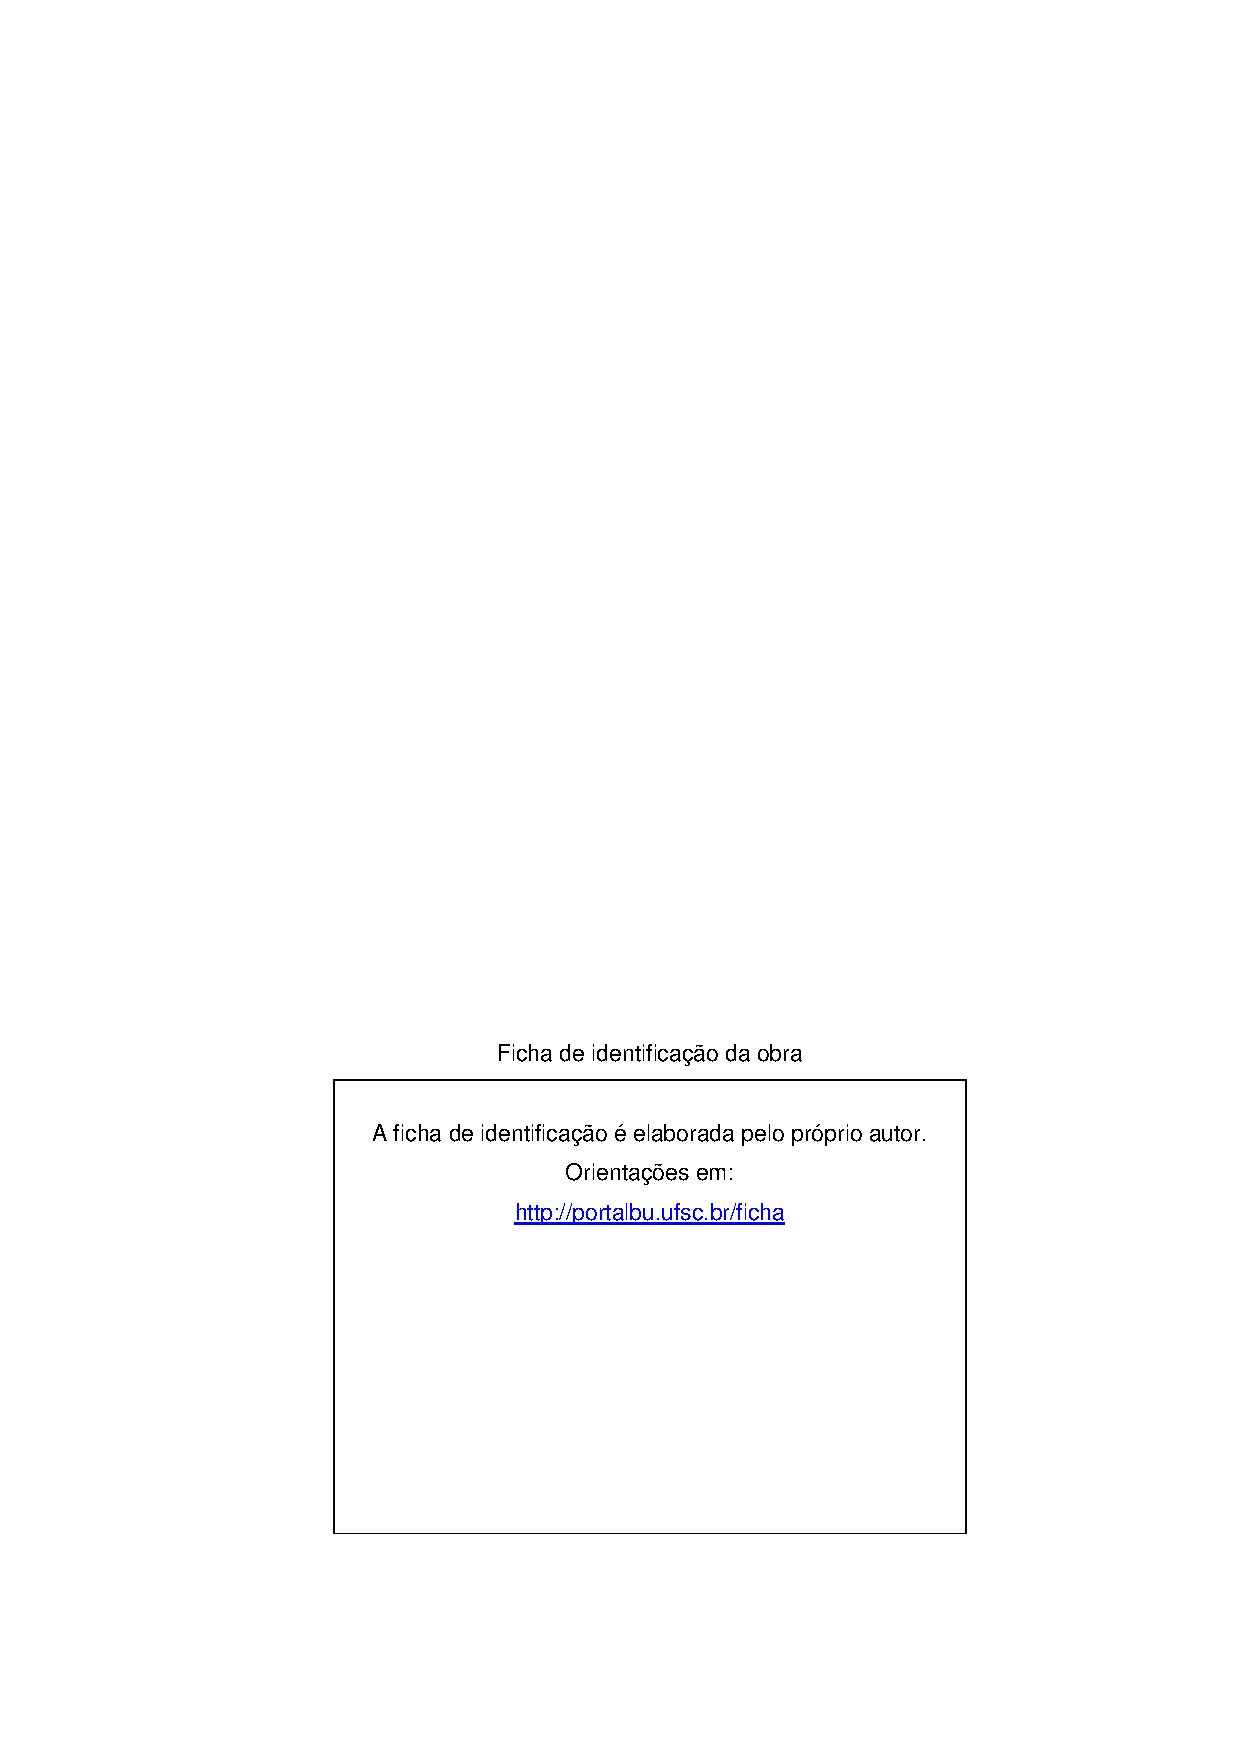
\includepdf{beforetext/Ficha_Catalografica.pdf}
\end{fichacatalografica}
% ---

% ---
% Inserir folha de aprovação
% ---
\begin{folhadeaprovacao}
	\OnehalfSpacing
	\centering
	\imprimirautor\\%
	\vspace*{10pt}		
	\textbf{\imprimirtitulo}%
	\ifnotempty{\imprimirsubtitulo}{:~\imprimirsubtitulo}\\%
	%		\vspace*{31.5pt}%3\baselineskip
	\vspace*{\baselineskip}
	
	Esta monografia foi julgada no contexto da disciplina DAS5511 (Projeto de Fim de Curso) e aprovada em sua forma final pelo \imprimircurso\\
	\vspace*{\baselineskip}
	Florianópolis, <dia(número)> de <mês> de <ano(número)>.\\
	
	%%%%%%%%%%%%%%%%%%%%%%%%%%%%%%%%%%%%%%%%%%%%%%%%%
	%IMPORTANTE: não é necessário assinaturas abaixo!
	%%%%%%%%%%%%%%%%%%%%%%%%%%%%%%%%%%%%%%%%%%%%%%%%%
	
	\vspace*{2\baselineskip}
	%\rule{0.4\textwidth}{0.4pt}\\
	Prof. Marcelo De Lellis Costa De Oliveira, Dr.\\
	Coordenador do Curso\\
	
	\vspace*{\baselineskip}
	\textbf{Banca Examinadora:} \\ \emph{[preencher somente após a defesa para a  Versão Final da BU]} \\
	
	
	\vspace*{2\baselineskip}
	%\rule{0.4\textwidth}{0.4pt}\\
	Prof(a). Carlos Barros Montez, Dr.\\
	Orientador(a) \\
	UFSC/CTC/EAS\\
	
	\vspace*{2\baselineskip}
	%\rule{0.4\textwidth}{0.4pt}\\
	Matheus Fischer, Eng.\\
	Supervisor(a) \\
	Fischertec Tecnologia\\
	
	\vspace*{2\baselineskip}
	%\rule{0.4\textwidth}{0.4pt}\\
	Prof(a). xxxx, Dr(a).\\
	Avaliador(a) \\
	Instituição xxxx\\
	
	\vspace*{2\baselineskip}
	%\rule{0.4\textwidth}{0.4pt}\\
	Prof. xxxx, Dr.\\
	Presidente da Banca \\
	UFSC/CTC/EAS
\end{folhadeaprovacao}
% ---

% ---
% Dedicatória
% ---
\begin{dedicatoria}
	\vspace*{\fill}
	\noindent
	\begin{adjustwidth*}{}{5.5cm} 
		\raggedleft
		Este trabalho é dedicado aos meus amigos, colegas de classe, namorada e aos meus queridos pais.
	\end{adjustwidth*}
\end{dedicatoria}
% ---

% ---
% Agradecimentos
% ---
\begin{agradecimentos}
	Primeiramente, expresso minha gratidão à minha família, que sempre me incentivou a seguir meus sonhos acadêmicos. Agradeço particularmente à minha mãe Sandra Vicenzi e meu pai Sergio Vicenzi, pelo seu amor incondicional e pela confiança depositada em mim. Também quero mencionar minha irmã Micheli e meu cunhado Matheus, que sempre me fornecem suporte e ajuda nas horas difíceis.

	Agradeço também à minha avó Vilma e à minha tia Samara e tio Celso, que sempre me inspiraram a manter o foco e buscar excelência em tudo que faço. Por fim, quero destacar minha namorada Monike, que compartilha comigo todo o amor e paciência durante os momentos mais ansiosos da minha trajetória acadêmica. Seu apoio foi essencial para manter me motivado e garantir que todo o trabalho fosse feito com qualidade e entusiasmo.

	Agradeço ao meus colegas de classe da turma da Automação 16.2, cuja amizade e colaboração fizeram toda a diferença no desenvolvimento deste projeto. Seus comentários e sugestões foram essenciais para refinar ideias e garantir que o trabalho fosse realizado com excelência. O apoio da turma foi fonte de inspiração para manter me motivado durante os momentos mais desafiadores.

	Em seguida, quero expressar minha gratidão pelo incrível suporte recebido por meu orientador acadêmico, Carlos Montez. Sua sabedoria, paciência e expertise foram fundamentais para guiar meus passos acadêmicos, permitindo que eu avançasse com confiança no caminho da excelência na pesquisa e desenvolvimento.

	Também quero agradecer ao meu supervisor Matheus Fischer por proporcionar o contexto prático da problemática estudada neste trabalho. Seu apoio foi crucial para garantir que a solução proposta estivesse alinhada com as necessidades reais da empresa e que fossem disponibilizadas todas as recursos necessários para a realização do projeto.

	Por fim, agradeço a todos os meus professores da Universidade Federal de Santa Catarina, que sempre compartilharam seus conhecimentos, garantindo a qualidade e rigor dos meus estudos. Suas contribuições foram fundamentais para o sucesso deste projeto.

\end{agradecimentos}
% ---

% ---
% Epígrafe
% ---
% \begin{epigrafe}
% 	\vspace*{\fill}
% 	\begin{flushright}
% 		\textit{``Texto da Epígrafe.\\
% 			Citação relativa ao tema do trabalho.\\
% 			É opcional. A epígrafe pode também aparecer\\
% 			na abertura de cada seção ou capítulo.\\
% 			Deve ser elaborada de acordo com a NBR 10520.''\\
% 			(SOBRENOME do autor da epígrafe, ano)}
% 	\end{flushright}
% \end{epigrafe}
% ---

% ---
% DECLARAÇÃO DE PUBLICIDADE
% ---

\begin{center}
	\textbf{DECLARAÇÃO DE PUBLICIDADE}
\end{center}

% Atenção: atualize o conteúdo de <texto>.

% <Nome da cidade>, <dia> de <mês> de <ano>.
Blumenau, 17 de janeiro de 2025.

\vspace{1cm}

Na condição de representante da <instituição de realização do PFC> na qual o presente trabalho foi realizado, declaro não haver ressalvas quanto ao aspecto de sigilo ou propriedade intelectual sobre as informações contidas neste documento, que impeçam a sua publicação por parte da Universidade Federal de Santa Catarina (UFSC) para acesso pelo público em geral, incluindo a sua disponibilização \emph{online} no Repositório Institucional da Biblioteca Universitária da UFSC. Além disso, declaro ciência de que o autor, na condição de estudante da UFSC, é obrigado a depositar este documento, por se tratar de um Trabalho de Conclusão de Curso, no referido Repositório Institucional, em atendimento à Resolução Normativa n° 126/2019/CUn.

Por estar de acordo com esses termos, subscrevo-me abaixo.

\vspace{15mm}

\begin{center}
	\rule{7cm}{0.7pt} \\
	Matheus Fischer, Eng. \\
	Fischertec Tecnologia
\end{center}

\cleardoublepage

% ---
% RESUMOS
% ---

% resumo em português
% \setlength{\absparsep}{18pt} % ajusta o espaçamento dos parágrafos do resumo
% \begin{resumo}
% 	\SingleSpacing
% 	\textbf{Instruções do padrão genérico de TCCs da BU:}
% 	No Resumo são ressaltados o objetivo da pesquisa, o método utilizado, as discussões e os resultados com destaque apenas para os pontos principais. O resumo deve ser significativo, composto de uma sequência de frases concisas, afirmativas, e não de uma enumeração de tópicos. Não deve conter citações. Deve usar o verbo na voz ativa e na terceira pessoa do singular. O texto do resumo deve ser digitado, em um único bloco, sem espaço de parágrafo. O espaçamento entre linhas é simples e o tamanho da fonte é 12. Abaixo do resumo, informar as palavras-chave (palavras ou expressões significativas retiradas do texto) ou, termos retirados de thesaurus da área. Deve conter de 150 a 500 palavras. O resumo é elaborado de acordo com a NBR 6028. 
	
% 	\textbf{Instruções da Coordenação de PFC:} O Resumo deve descrever de forma sucinta: o contexto/motivação/problema tratado no PFC; a solução proposta; a implementação/desenvolvimento; a metodologia e as principais técnicas e ferramentas utilizadas; os principais resultados obtidos e a importância/impactos de tais resultados para a empresa/clientes da empresa/instituto de pesquisa. Escrever todos esses pontos de forma bem resumida e direta, e sem entrar em detalhes técnicos. O tamanho do Resumo deve ocupar praticamente esta página inteira, e num \textbf{único} parágrafo. Além disso, Resumo + Palavras-Chave não podem ultrapassar esta página. 
		
% 	\textbf{Palavras-chave}: Palavra-chave 1. Palavra-chave 2. Palavra-chave 3. \emph{[essas palavras-chave devem obrigatoriamente ser utilizadas no Resumo]}
% \end{resumo}
\setlength{\absparsep}{18pt} % ajusta o espaçamento dos parágrafos do resumo
\begin{resumo}
	\SingleSpacing
	A Fischertec Tecnologia é uma empresa brasileira que se concentra no desenvolvimento de soluções digitais de alta qualidade. Atua no setor de sites, aplicativos, e-commerces e diversos produtos digitais, buscando transformar ideias em soluções bem projetadas e inovadoras.

	O principal objetivo deste PFC é criar um MVP (Minimum Viable Product) de uma plataforma de agendamento de reservas de quadras esportivas em uma aplicação SaaS (\textit{Software as a Service}). A criação desse sistema foi motivada pelas demandas específicas das empresas esportivas, como personalização de horários, preços e integrações com dispositivos IoT.

	A Fischertec busca fornecer uma solução robusta, eficiente e alinhada às melhores práticas de automação e gestão esportiva. Ela optou por desenvolver um sistema proprietário que ofereça a experiência dos clientes empresariais com um produto único e personalizável, em busca da redução de sua dependência de projetos externos.

	O desenvolvimento da aplicação do servidor, que é o escopo deste PFC, utiliza Nest.js para a API REST, PostgreSQL como banco de dados e Docker para conteinerização. O sistema frontend, em Next.js/React, será responsável pela interface do usuário em um futuro desenvolvimento. A metodologia utilizada foi ágil, garantindo entregas iterativas e validações frequentes com o TypeORM para persistência de dados. Postman serve como ferramenta de testes da API.

	O principal resultado obtido é a entrega de uma aplicação backend totalmente funcional que permite o gerenciamento completo de locações, com autenticação e controle de usuários e papéis para diferentes \textit{tenants} e preparada para uma futura integração com interface gráfica web. O sistema se mostrou eficiente, alinhado aos objetivos propostos e de fácil usabilidade.

	A aplicação do servidor é totalmente original e inovadora, destacando-se na resolução dos problemas enfrentados pela Fischertec ao simular um cenário real de operação.

	\textbf{Palavras-chave}: SaaS. Nest.js. IoT. Desenvolvimento. Software. Backend. Quadras. Esportivas. Gerenciamento. Agendamento
\end{resumo}

% % resumo em inglês
% \begin{resumo}[Abstract]
% 	\SingleSpacing
% 	\begin{otherlanguage*}{english}
% 		Resumo traduzido para outros idiomas, neste caso, inglês. Segue o formato do resumo feito na língua vernácula. As palavras-chave traduzidas, versão em língua estrangeira, são colocadas abaixo do texto precedidas pela expressão “Keywords”, separadas por ponto.
		
% 		\textbf{Keywords}: Keyword 1. Keyword 2. Keyword 3.
% 	\end{otherlanguage*}
% \end{resumo}

% resumo em inglês
\begin{resumo}[Abstract]
	\SingleSpacing
	\begin{otherlanguage*}{english}
		The Fischertec Tecnologia is a Brazilian company focused on providing high-quality digital solutions. It operates in the fields of websites, applications, e-commerce, and various digital products, with a focus on transforming ideas into well-designed and innovative solutions.

		The main objective of this PFC is to create a MVP (Minimum Viable Product) of a sports fields reservations management platform in a SaaS environment. The creation of this system was motivated by the specific needs of sports industry companies, such as customizable schedules, prices, and IoT device integrations.

		The Fischertec company aims to provide a robust, efficient, and aligned with best practices solution for sports enthusiasts by offering an unique and personalized product experience. They opted to develop an owner-owned solution that aims to reduce their dependency on external projects.
		During this PFC project, the server application development scope is focused. It uses Nest.js for the REST API, PostgreSQL as the database, and Docker for containerization. The frontend system in Next.js/React will be responsible for the graphical user interface in a future development.
		The methodology used was agile, ensuring iterative deliveries and frequent validations with TypeORM for data persistence. Postman is used as a tool for testing the API.
		The main result obtained is the delivery of a fully functional backend application that allows comprehensive management and booking/scheduling of sports locations, with authentication and user roles for different tenants. The system was efficient and aligned with the proposed objectives and easy to use.

		The server-side application is original and innovative, standing out in the resolution of issues faced by the Fischertec company through simulating a real operation scenario.
		
		\textbf{Keywords}: SaaS. Nest.js. IoT. Development. Software. Backend. Fields. Sports. Management. Booking. Scheduling.
	\end{otherlanguage*}
\end{resumo}

%% resumo em francês 
%\begin{resumo}[Résumé]
% \begin{otherlanguage*}{french}
%    Il s'agit d'un résumé en français.
% 
%   \textbf{Mots-clés}: latex. abntex. publication de textes.
% \end{otherlanguage*}
%\end{resumo}
%
%% resumo em espanhol
%\begin{resumo}[Resumen]
% \begin{otherlanguage*}{spanish}
%   Este es el resumen en español.
%  
%   \textbf{Palabras clave}: latex. abntex. publicación de textos.
% \end{otherlanguage*}
%\end{resumo}
%% ---

{%hidelinks
	\hypersetup{hidelinks}
	% ---
	% inserir lista de ilustrações
	% ---
	\pdfbookmark[0]{\listfigurename}{lof}
	\listoffigures*
	\cleardoublepage
	% ---
	
	% ---
	% inserir lista de quadros
	% ---
	% \pdfbookmark[0]{\listofquadrosname}{loq}
	% \listofquadros*
	% \cleardoublepage
	% ---
	
	% ---
	% inserir lista de tabelas
	% ---
	\pdfbookmark[0]{\listtablename}{lot}
	\listoftables*
	\cleardoublepage
	% ---
	
	% ---
	% inserir lista de abreviaturas e siglas (devem ser declarados no preambulo)
	% ---
	\imprimirlistadesiglas
	% ---
	
	% ---
	% inserir lista de símbolos (devem ser declarados no preambulo)
	% ---
	\imprimirlistadesimbolos
	% ---
	
	% ---
	% inserir o sumario
	% ---
	\pdfbookmark[0]{\contentsname}{toc}
	\tableofcontents*
	\cleardoublepage
	
}%hidelinks
% ---
% ---

% ----------------------------------------------------------
% ELEMENTOS TEXTUAIS
% ----------------------------------------------------------
\textual

% ---
% 1 - Introdução
% ---
% ----------------------------------------------------------
\chapter{Introdução}
% ----------------------------------------------------------

% \textbf{Instruções do padrão genérico de TCCs da BU:} 

% As orientações aqui apresentadas são baseadas em um conjunto de normas elaboradas pela \gls{ABNT}. Além das normas técnicas, a Biblioteca também elaborou uma série de tutoriais, guias, \textit{templates} os quais estão disponíveis em seu site, no endereço \url{http://portal.bu.ufsc.br/normalizacao/}.

% Paralelamente ao uso deste \textit{template} recomenda-se que seja utilizado o \textbf{Tutorial de Trabalhos Acadêmicos} (disponível neste link \url{https://repositorio.ufsc.br/handle/123456789/180829}).

% Este \textit{template} está configurado apenas para a impressão utilizando o anverso das folhas, caso você queira imprimir usando a frente e o verso, acrescente a opção \textit{openright} e mude de \textit{oneside} para \textit{twoside} nas configurações da classe \textit{abntex2} no início do arquivo principal \textit{main.tex} \cite{abntex2classe}.

% Conforme a \href{https://repositorio.ufsc.br/bitstream/handle/123456789/197121/RN46.2019.pdf?sequence=1&isAllowed=y}{Resolução NORMATIVA nº 46/2019/CPG} as dissertações e teses não serão mais entregues em formato impresso na Biblioteca Universitária. Consulte o Repositório Institucional da UFSC ou sua Secretaria de Pós Graduação sobre os procedimentos para a entrega. 

% \nocite{NBR6023:2002}
% \nocite{NBR6027:2012}
% \nocite{NBR6028:2003}
% \nocite{NBR10520:2002}

% \textbf{Instruções da Coordenação do PFC:} 

% A Introdução deve apresentar um panorama geral do PFC de modo resumido, sem entrar em detalhes técnicos, para que o leitor já entenda aqui na Introdução o começo, meio e fim do PFC. Assim, é muito importante deixar bem claro na Introdução os seguintes pontos (a Introdução pode ser vista como um resumo geral do PFC, e a Seção Resumo como um resumo desse resumo): 

% \begin{itemize}
%      \item O contexto e a motivação do PFC, com uma breve descrição da empresa/instituto de pesquisa (histórico, clientes, produtos, serviços, projetos, etc) em que o PFC foi realizado e do projeto global da empresa em que o PFC está inserido (se for o caso)
%      \item Breve descrição do problema tratado no PFC;
%     \item A importância de tal problema para a empresa/clientes da empresa/instituto de pesquisa;
%     \item Objetivos: aqui são descritos os objetivos, que podem ser estratificados em objetivo geral e objetivos específicos. Outra opção é colocar os objetivos específicos na forma de passos de uma metodologia de trabalho, ou seja, os procedimentos e ferramentas adotadas em cada fase do projeto (um plano de trabalho).
%     \item Breve descrição da solução proposta;
%     \item Breve descrição da implementação/desenvolvimento realizado;
%     \item Breve descrição da metodologia e das principais técnicas e ferramentas utilizadas (do ponto de vista técnico). \textbf{Importante}: como \emph{Scrum} é uma metodologia geral de execução de projetos, ele não se enquadra aqui, pois não se trata de uma metodologia técnica específica para o desenvolvimento do PFC;
%     \item Breve descrição dos principais resultados obtidos e da importância/impactos de tais resultados para a empresa/clientes da empresa/instituto de pesquisa;
%     \item Deixar bem claro o que foi de fato foi realizado pelo(a) autor(a), diferenciando do que foi aproveitado de trabalhos anteriores/outras times da empresa. \textbf{Importante}: esta preocupação em diferenciar o trabalho realizado pelo(a) autor(a) daquele de possíveis colegas de um time deve permear todo o documento.
% \end{itemize}

% Ressaltamos a seguir alguns aspectos cruciais para a escrita do PFC:
% \begin{itemize}
% 	\item Apesar de o tamanho da monografia não ter uma correlação direta com a nota, bons trabalhos costumam ter de 60 a 70 páginas efetivamente escritas (desde a Introdução até a Conclusão, excluindo-se Capa, Resumo, Sumário, Referências Bibliográficas, etc).  Por outro lado, acima de 100 páginas a monografia pode se tornar ``massante'', discorrendo além do necessário para o entendimento do trabalho e, consequentemente, perdendo o foco do leitor.
% 	\item A linguagem a ser utilizada em um trabalho acadêmico deve ser técnico-científica e, portanto, formal (e não informal, como se o trabalho estivesse sendo explicado a um colega ou familiar). Desse modo, não devem ser usadas gírias. Além disso, não se deve escrever ``o trabalho feito por mim'', mas sim algo como ``o presente trabalho trata de/o trabalho realizado pelo(a) autor(a)/etc''.
% 	\item Utilize corretor ortográfico, verifique a gramática, e revise com muito cuidado e atenção todo o texto: pontuação, uso da vírgula, concordância, coesão e clareza textual, encadeamento entre frases, sentenças e parágrafos, etc.
% 	\item Este documento deve corresponder a uma monografia acadêmica, em que se deve fundamentar e justificar as ideias, afirmações, métodos e deduções apresentadas com base em técnicas, ferramentas, metodologias, equações, normas, literatura especializada (livros e artigos), etc, e não a um relatório descritivo voltado a um departamento/time de uma empresa. 
% 	\item As referências bibliográficas não podem conter apenas sites, blogs e manuais técnicos: devem também conter livros, artigos, dissertações, teses, etc. Além disso, há uma diferença entre citação \emph{direta} (comando \verb!\citeas!) e citação \emph{indireta} (comando \verb!\cite!).
% \end{itemize}

% \section*{Estrutura do documento}

% Ao final da Introdução (que é o Capítulo 1), costuma-se apresentar como o documento está organizado, descrevendo brevemente o que é tratado nos demais capítulos do Sumário, começando pelo Capítulo 2. A estrutura de capítulos mostrada no Sumário deste documento é apenas uma sugestão geral e não precisa ser seguida à risca: dependendo da área e do foco do trabalho, tanto a estrutura detalhada (Capítulos, Seções e Subseções) quanto o número de capítulos pode variar. O(A) estudante deve consultar seu(sua) Orientador(a) Acadêmico(a) para definir a estrutura detalhada do documento.

% \noindent\textbf{Exemplo}:

% \emph{O presente documento está organizado da seguinte maneira. O Capítulo~2 apresenta a fundamentação teórica sobre os principais conceitos e técnicas necessárias para o entendimento do problema abordado e da solução proposta. O problema tratado neste PFC é descrito em detalhes no Capítulo~3, juntamente com os requisitos técnicos a serem atendidos. O Capítulo~4 aborda a solução proposta e a metodologia envolvida. O desenvolvimento realizado e a análise dos resultados obtidos são mostrados no Capítulo~5. Por fim, no Capítulo~6, são apresentadas as conclusões deste trabalho e algumas sugestões de trabalhos futuros são elencadas.}

A situação atual das empresas que administram quadras esportivas revela uma crescente demanda por sistemas de agendamento e controle de reservas mais eficientes e automatizados. Com o aumento da competitividade no setor, essas empresas buscam soluções que não apenas organizem os horários e disponibilidades de seus espaços, mas que também integrem funcionalidades de automação de dispositivos, como iluminação, climatização e sistemas de acesso. A automação integrada aos agendamentos é crucial para reduzir desperdícios de energia e otimizar os custos operacionais, permitindo que os dispositivos sejam acionados apenas nos horários em que as quadras estão efetivamente em uso. Além disso, essas práticas têm um impacto positivo no meio ambiente, reduzindo a pegada de carbono das operações e promovendo um modelo de negócio mais sustentável.

\section{A Empresa Fischertec}

A Fischertec Tecnologia é uma empresa dedicada a transformar ideias em soluções digitais de alta qualidade. Atua no desenvolvimento de sites, aplicativos, e-commerce e diversos produtos digitais, sempre focando em inovação e excelência.

A empresa conta com uma equipe de especialistas em design e desenvolvimento. Os designers são experientes em UX/UI e dedicados a criar interfaces que proporcionem a melhor experiência ao usuário. Os desenvolvedores fullstack da equipe da Fischertec têm expertise em diversas tecnologias e frameworks, garantindo a entrega de soluções robustas e eficazes.

A Fischertec, buscando criar um produto próprio com o objetivo de reduzir sua dependência de projetos externos, optou por desenvolver um sistema de gerenciamento de reservas de quadras esportivas. A decisão de desenvolver esse sistema foi motivada pela necessidade de atender demandas específicas das empresas esportivas, como personalização de horários, preços e integrações com dispositivos IoT. A criação de um sistema proprietário também reflete a estratégia da Fischertec de se posicionar como referência no setor, oferecendo uma solução robusta, eficiente e alinhada às melhores práticas de automação e gestão esportiva.

\section{O Problema e os Objetivos}

O problema central abordado é a dificuldade em gerenciar reservas de forma integrada e eficiente, definindo horários de funcionamento, preços de locação, tipos de quadras disponíveis entre outras opções. Essa dificuldade impacta diretamente a experiência dos clientes, bem como a eficiência administrativa da empresa.

O objetivo geral do projeto foi desenvolver um \gls{MVP} de uma plataforma que permita gerenciar reservas de quadras esportivas de forma centralizada, disponível na web e personalizável para diferentes empresas. Foram estabelecidos alguns objetivos específicos:

\begin{itemize}
    \item A criação de um sistema com autenticação de usuários;
    \item Controle de permissões de usuário baseado em papéis e configurável para diferentes \textit{tenants};
    \item Definição e gerenciamento de quadras com possibilidade de personalização, como tipos de quadras, preços e horários de funcionamento;
    \item Configuração do \textit{tenant} da empresa, com nome e horários de funcionamento;
    \item Agendamento de reservas com controle de disponibilidade;
    \item Integração com dispositivos IoT para automação de recursos presentes nas quadras de acordo com as reservas.
\end{itemize}

A Fischertec busca fornecer uma solução que otimize os processos operacionais e ofereça uma experiência mais eficiente e moderna para seus clientes empresariais, com foco nos esportistas que utilizam quadras esportivas e participam de aulas coletivas. Portanto, foi proposta uma solução que envolveu o desenvolvimento de uma aplicação web composta por um servidor com API REST e um sistema \textit{frontend}, ambos projetados para oferecer flexibilidade e desempenho. O sistema foi implementado utilizando uma arquitetura modular baseada em camadas, promovendo a separação de responsabilidades e facilitando futuras manutenções e expansões. Foram utilizadas tecnologias modernas, como Nest.js para a API, PostgreSQL para o banco de dados e Docker para conteinerização. A interface web será futuramente desenvolvida em Next.js/React. Além disso, houve integração com a plataforma IoT eWeLink da Shenzhen Coolkit Technology CO., LTD, possibilitando o controle automatizado de dispositivos associados às quadras.

A metodologia aplicada ao desenvolvimento seguiu práticas ágeis, garantindo entregas iterativas e validações frequentes. Ferramentas como Postman foram utilizadas para testes das APIs, enquanto o TypeORM auxiliou na persistência dos dados. O desenvolvimento foi estruturado de modo a criar um sistema totalmente funcional e alinhado com os objetivos propostos. Devido à maior complexidade, optou-se por focar no desenvolvimento da aplicação do servidor, que é o escopo deste PFC.

Os principais resultados obtidos incluem a entrega de uma aplicação \textit{backend} que permite o gerenciamento completo de locações, com controle de usuários e papéis para diferentes \textit{tentants} (locatários), gerenciamento de horários e automação de dispositivos IoT no início e fim das reservas. O sistema se mostrou eficiente e de fácil usabilidade, atendendo às expectativas da Fischertec ao simular um cenário real de operação. 

Todo o desenvolvimento da aplicação do servidor foi realizado pelo autor, sem aproveitamento direto de trabalhos prévios ou de outros times, o que reforça o caráter original e inovador do projeto. A aplicação cumpre o objetivo de resolver os problemas de gerenciamento enfrentados pela Fischertec, destacando-se como uma solução escalável e tecnológica para o setor.

\section{Estrutura do documento}

O presente documento está organizado da seguinte maneira. O \autoref{cap:fundamentacao_teorica} apresenta a fundamentação teórica sobre os principais conceitos e técnicas necessárias para o entendimento do problema abordado e da solução proposta. O problema tratado neste PFC é descrito em detalhes no \autoref{cap:descricao_problema_e_requisitos}, juntamente com os requisitos técnicos a serem atendidos. No \autoref{cap:solucao_proposta} é explicada a solução proposta e a metodologia utilizada. O \autoref{cap:desenvolvimento_e_analise_resultados} aborda o desenvolvimento da solução proposta incluindo as tecnologias utilizadas e a análise dos resultados obtidos. Por fim, no \autoref{cap:conclusao}, são apresentadas as conclusões deste trabalho e algumas sugestões de trabalhos futuros são elencadas.
% ---

% ---
% 2 - Capítulo 2
% ---
% ----------------------------------------------------------
\chapter{Fundamentação Teórica}\label{cap:fundamentacao_teorica}
% ----------------------------------------------------------

% \textbf{Instruções da Coordenação do PFC:}

% Deve-se colocar um parágrafo introdutório no início de \textbf{cada} capítulo, descrevendo os assuntos que serão abordados e a relação com o restante do trabalho. Por exemplo: \emph{A Seção 2.1 apresenta \ldots. Os resultados obtidos são analisados na Seção 2.2.} Pode-se fazer o mesmo no início de seções maiores, explicando para o leitor, em uma ou duas sentenças, o que está por vir no texto e o porquê. Outra boa prática é, ao final de cada capítulo, fazer uma ligação com o capítulo seguinte por meio de parágrafo curto.

% Neste capítulo, deve-se apresentar as principais teorias, conceitos, técnicas, modelos, etc que são essenciais para o entendimento do problema tratado e da solução proposta.

% Figuras, tabelas, quadros e equações devem ser introduzidos e explicados no texto: não se pode simplesmente ``jogá-los'' no texto, sem referência nem explicação. Por exemplo, deve-se escrever algo como: \emph{O circuito projetado é mostrado na Figura~10. O resistor $R_1$ faz o papel de um limitador de corrente, enquanto o capacitor $C_2$ juntamente com o resistor $R_5$ formam um filtro passa-baixa. Este circuito tem a vantagem de \ldots}

% Com relação às equações, não se faz referência a uma equação que ainda não foi apresentada. Por exemplo, não se escreve: \emph{A relação entre a tensão e a corrente de um resistor é dada pela \autoref{eq:leiDeOhm}:}
% \begin{equation}\label{eq:leiDeOhm}
%     V = R I \, \text{.}
% \end{equation}

% \noindent O correto é algo como: \emph{A relação entre a tensão e a corrente de um resistor é dada por (Lei de Ohm)}
% \begin{equation}\label{eq:leiDeOhm2}
%     V = R I \, \text{,}
%    \end{equation}
% \emph{na qual $V$ é a tensão sobre o resistor, $R$ a resistência e $I$ a corrente elétrica. Da \autoref{eq:leiDeOhm2}, obtemos que}
% \begin{equation}\label{eq:leiDeOhm3}
%     I = \dfrac{V}{R} \, \text{.}
% \end{equation}

% \emph{Por outro lado, \ldots}

% É importante observar que as equações fazem parte do texto e, assim, deve-se inserir uma vírgula ou ponto ao seu final. Se o parágrafo segue, pode-se eliminar o recuo na próxima linha com o comando \verb!\noindent!. Além disto, se a frase segue, inicia-se a linha com letra minúscula. Veja os exemplos das Equações~(\ref{eq:leiDeOhm2}) e (\ref{eq:leiDeOhm3}).

% A seguir encontra-se uma equação na linha de texto: $\hat{y}(t+k\mid t)= \sum^\infty_{i=1} g_i \Delta u(t+k-i\mid t)$. E também, mais à frente, um exemplo de referência cruzada da \autoref{fig:Fig_1} e da \autoref{eq:Eq_1}.

% \pagebreak

% \textbf{Instruções do padrão genérico de TCCs da BU:}

% Deve-se inserir texto entre as seções.

% % ----------------------------------------------------------
% \section{Exposição do tema ou matéria}
% % ----------------------------------------------------------

% É a parte principal e mais extensa do trabalho. Deve apresentar a fundamentação teórica, a metodologia, os resultados e a discussão. Divide-se em seções e subseções conforme a NBR 6024 \cite{NBR6024:2012}.

% Quanto à sua estrutura e projeto gráfico, segue as recomendações da \gls{ABNT} para preparação de trabalhos acadêmicos, a NBR 14724, de 2011 \cite{NBR14724:2011}.

% \begin{figure}[htb]
% 	\caption{\label{fig:Fig_1}Elementos do trabalho acadêmico.}
% 	\begin{center}
% 		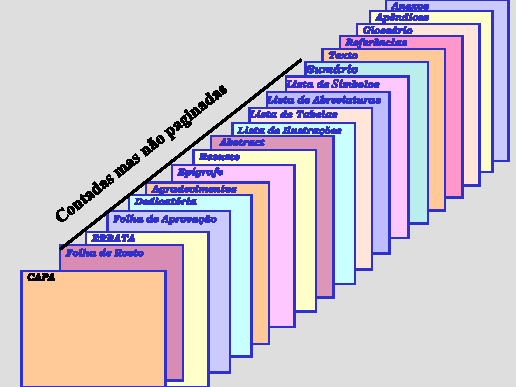
\includegraphics{images/imagem.pdf}
% 	\end{center}
% 	\fonte{Universidade Federal do Paraná (1996).}
% \end{figure}

% % ----------------------------------------------------------
% \subsection{Formatação do texto}
% % ----------------------------------------------------------

% No que diz respeito à estrutura do trabalho, recomenda-se que:
% \begin{alineas}
% 	\item o texto deve ser justificado, digitado em cor preta, podendo utilizar outras cores somente para as ilustrações;
% 	\item utilizar papel branco ou reciclado para impressão;
% 	\item os elementos pré-textuais devem iniciar no anverso da folha, com exceção da ficha catalográfica ou ficha de identificação da obra;
% 	\item os elementos textuais e pós-textuais devem ser digitados no anverso e verso das folhas, quando o trabalho for impresso. As seções primárias devem começar sempre em páginas ímpares, quando o trabalho for impresso. Deixar um espaço entre o título da seção/subseção e o texto e entre o texto e o título da subseção.
% \end{alineas}

% No \autoref{qua:Quadro_1} estão as especificações para a formatação do texto.

\begin{quadro}[htb]
	\centering
	\caption{\label{qua:Quadro_1}Formatação do texto.}	
	\begin{tabular}{|l|p{11cm}|}
		\hline
		\textbf{Formato do papel} & A4.\\ \hline
		\textbf{Impressão}        & A norma recomenda que caso seja necessário imprimir, deve-se utilizar a frente e o verso da página.\\ \hline
		\textbf{Margens}          & Superior: 3, Inferior: 2, Interna: 3 e Externa: 2. Usar margens espelhadas quando o  trabalho for impresso.\\ \hline
		\textbf{Paginação}        & As páginas dos elementos pré-textuais devem ser contadas, mas não numeradas. Para trabalhos digitados somente no anverso, a numeração das páginas deve constar no canto superior direito da página, a 2 cm da borda, figurando a partir da primeira folha da  parte textual. Para trabalhos digitados no anverso e no verso, a numeração deve constar no canto superior direito, no anverso, e no canto superior esquerdo no verso.\\ \hline
		\textbf{Espaçamento}      & O texto deve ser redigido com espaçamento entre linhas 1,5, excetuando-se as citações de mais de três linhas, notas de rodapé, referências, legendas das ilustrações e das tabelas, natureza (tipo do trabalho, objetivo, nome da instituição a que é submetido e área de concentração), que devem ser digitados em espaço simples, com fonte menor. As referências devem ser separadas entre si por um espaço simples em branco.\\ \hline
		\textbf{Paginação}        & A contagem inicia na folha de rosto, mas se insere o número da página na introdução até o final do trabalho.\\ \hline
		\textbf{Fontes sugeridas} & Arial ou Times New Roman.\\ \hline
		\textbf{Tamanho da fonte} & \textbf{Fonte tamanho 12 para o texto}, incluindo os títulos das seções e subseções. As citações com mais de três linhas, notas de rodapé, paginação, dados internacionais de catalogação, legendas e fontes das ilustrações e das tabelas devem ser de tamanho menor. Adotamos, neste \textit{template} \textbf{fonte tamanho 10}.\\ \hline
		\textbf{Nota de rodapé}   & Devem ser digitadas dentro da margem, ficando separadas por um espaço simples por entre as linhas e por filete de 5 cm a partir da margem esquerda. A partir da segunda linha, devem ser alinhadas embaixo da primeira letra da primeira palavra da primeira linha.\\ \hline
	\end{tabular}
	\fonte{\textcite{NBR14724:2011}.}
\end{quadro}

% % ----------------------------------------------------------
% \subsubsection{As ilustrações}
% % ----------------------------------------------------------

% Independentemente do tipo de ilustração (quadro, desenho, figura, fotografia, mapa, entre outros), a sua identificação aparece na parte superior, precedida da palavra designativa. 

% \begin{citacao}
% 	Após a ilustração, na parte inferior, indicar a fonte consultada (elemento obrigatório, mesmo que seja produção do próprio autor), legenda, notas e outras informações necessárias à sua compreensão (se houver). A ilustração deve ser citada no texto e inserida o mais próximo possível do texto a que se refere. \cite[p. 11]{NBR14724:2011}.
% \end{citacao}

% % ----------------------------------------------------------
% \subsubsection{Equações e fórmulas}
% % ----------------------------------------------------------

% As equações e fórmulas devem ser destacadas no texto para facilitar a leitura.  Para numerá-las, usar algarismos arábicos entre parênteses e alinhados à direita. Pode-se adotar uma entrelinha maior do que a usada no texto \cite{NBR14724:2011}.

% Exemplos, \autoref{eq:Eq_1} e \autoref{eq:Eq_2}. Observe que o comando \verb|\gls{}| é usado para utilizar para criar um \emph{hyperlink} com a definição do símbolo na lista de símbolos (veja linha 153 de \emph{main.tex}.

% \begin{equation}
% \label{eq:Eq_1}
% \gls{C} = 2 \gls{pi} \gls{r} \sqrt{\gamma} + 10 \, \text{.}
% \end{equation}

% \begin{equation}
% \label{eq:Eq_2}
% \gls{A} = \gls{pi} \gls{r}^2 \, \text{.}
% \end{equation}

% \noindent Aqui não há recuo porque o parágrafo não terminou, apenas foi iniciada uma nova frase após a equação. As equações fazem parte do texto, portanto estão sujeitas à pontuação (ponto final, vírgula etc.).

% % ----------------------------------------------------------
% \subsubsubsection{Exemplo tabela}
% % ----------------------------------------------------------

% De acordo com \textcite{ibge1993}, tabela é uma forma não discursiva de apresentar informações em que os números representam a informação central. Ver \autoref{tab:Tab_1}.

% \begin{table}[htb]
% 	\ABNTEXfontereduzida
% 	\caption{\label{tab:Tab_1}Médias concentrações urbanas 2010-2011.}
% 	\begin{tabular}{@{}p{3.0cm}p{1.5cm}p{2cm}p{2.5cm}p{2.5cm}p{2.5cm}@{}}
% 		\toprule
% 		\textbf{Média concentração urbana} & \multicolumn{2}{l}{\textbf{População}} & \textbf{Produto Interno Bruto – PIB (bilhões R\$)} & \textbf{Número de empresas} & \textbf{Número de unidades locais} \\ \midrule
% 		\textbf{Nome}                      & \textbf{Total}   & \textbf{No Brasil}  &                                                   &                             & \\
% 		Ji-Paraná (RO)                     & 116 610          & 116 610             & 1,686                                             & 2 734                       & 3 082 \\
% 		Parintins (AM)                     & 102 033          & 102 033             & 0,675                                             & 634                         & 683 \\
% 		Boa Vista (RR)                     & 298 215          & 298 215             & 4,823                                             & 4 852                       & 5 187 \\
% 		Bragança (PA)                      & 113 227          & 113 227             & 0,452                                             & 654                         & 686 \\ \bottomrule
% 	\end{tabular}
% 	\fonte{\textcite{ibge2016}.}
% \end{table}

\section{APIs e APIs Restful}

APIs (\textit{Application Programming Interfaces}) são interfaces que permitem a comunicação entre diferentes sistemas, softwares ou componentes. Elas funcionam como pontes que facilitam o intercâmbio de dados e funcionalidades, promovendo integração e interoperabilidade. A ideia de API remonta aos primórdios da computação, quando surgiram as primeiras necessidades de criar padrões para que sistemas independentes pudessem se comunicar. Inicialmente, as APIs eram utilizadas em bibliotecas locais para abstrair funcionalidades complexas de hardware e software. Com o avanço da internet, especialmente nas décadas de 1990 e 2000, as APIs evoluíram para um modelo remoto, permitindo que sistemas distribuídos interagissem de maneira mais eficiente.

Nesse contexto, surgiu o conceito de APIs REST, um estilo arquitetural proposto por Roy Fielding em sua tese de doutorado em 2000. REST, acrônimo para \textit{Representational State Transfer}, baseia-se em princípios como uniformidade, ausência de estado (\textit{statelessness}), utilização de métodos HTTP - \textit{Hypertext Transfer Protocol} (GET, POST, PUT, DELETE, etc.), e representação de recursos por meio de URLs (\textit{Universal Resource Locators}). Fielding idealizou REST como uma maneira de padronizar a comunicação entre sistemas na web, tirando proveito das funcionalidades já existentes no protocolo HTTP. APIs REST ganharam popularidade devido à sua simplicidade, flexibilidade e capacidade de escalar, sendo amplamente adotadas por grandes empresas como Google, Twitter e Facebook \cite{fielding2000}.

A ligação entre APIs de forma geral e APIs REST está na evolução das necessidades de integração entre sistemas. Enquanto APIs genéricas servem como um conceito abrangente para qualquer forma de comunicação programada entre sistemas, as APIs REST trouxeram um conjunto específico de diretrizes para implementar essas interações de maneira eficiente e alinhada com os padrões da web. Ao adotar REST, as empresas passaram a criar interfaces mais padronizadas e acessíveis, o que facilitou a interoperabilidade entre sistemas desenvolvidos por diferentes organizações.

As vantagens de utilizar APIs, de modo geral, incluem a possibilidade de reuso de funcionalidades, redução de redundâncias no desenvolvimento e facilidade de integração entre diferentes tecnologias. Já as APIs REST se destacam por sua simplicidade e aderência aos padrões da web, tornando-as fáceis de implementar e consumir. Por serem baseadas em HTTP, um protocolo amplamente suportado, as APIs REST são agnósticas em relação à linguagem de programação e oferecem suporte para uma ampla gama de clientes, desde navegadores até dispositivos IoT \textit{(Internet das Coisas)}.

No livro "REST API Design Rulebook", Mark Masse destaca a importância de seguir boas práticas no design de APIs REST: "Uma API RESTful bem projetada deve ter como objetivo fornecer uma interface limpa e intuitiva para que os desenvolvedores interajam com recursos e serviços" \cite{masse2011rest}. Essa ênfase na simplicidade e clareza reflete as razões pelas quais APIs REST têm sido tão amplamente adotadas. Além de facilitar a integração entre sistemas, elas promovem a consistência no design, o que reduz a curva de aprendizado para desenvolvedores e aumenta a produtividade nas equipes de desenvolvimento. Assim, APIs e APIs REST desempenham um papel fundamental no desenvolvimento de soluções modernas e escaláveis, sendo uma base sólida para a inovação tecnológica.

\section{Cloud Computing}

A computação em nuvem, ou \textit{Cloud Computing}, é um modelo de fornecimento de recursos computacionais, como armazenamento, processamento, bancos de dados e softwares, por meio da internet. A ideia de disponibilizar recursos computacionais de maneira remota surgiu na década de 1960, com o conceito de \textit{time-sharing}, promovido por empresas como IBM e pesquisadores como John McCarthy, que previu que a computação poderia um dia ser organizada como um serviço público. No entanto, a computação em nuvem, como conhecida atualmente, começou a tomar forma nos anos 2000, com o surgimento de grandes provedores de serviços de nuvem, como Amazon Web Services (AWS), Microsoft Azure e Google Cloud Platform (GCP). A AWS, lançada em 2006, é amplamente reconhecida por popularizar a computação em nuvem com serviços como EC2 e S3, que forneceram acesso flexível e escalável a servidores e armazenamento.

Sobre a computação em núvem, Erl, Puttini e Mahmood, afirmam que:
\begin{citacao}
	A computação em nuvem representa uma mudança significativa na forma como os recursos de TI são projetados, implantados e gerenciados, oferecendo um modelo para permitir acesso de rede conveniente e sob demanda a um conjunto compartilhado de recursos de computação configuráveis \cite{Erl2013}.
\end{citacao}

Na atualidade, a computação em nuvem desempenha um papel essencial no desenvolvimento de software, especialmente no contexto de aplicações web e soluções de Internet das Coisas (IoT). No desenvolvimento de software web, a nuvem permite que empresas de todos os tamanhos utilizem infraestrutura escalável para hospedar seus aplicativos, garantindo alta disponibilidade e desempenho. Por exemplo, plataformas como AWS Elastic Beanstalk e Google App Engine facilitam a implantação e o gerenciamento de aplicativos web, reduzindo a complexidade da configuração de servidores. Além disso, ferramentas de integração e entrega contínuas (CI/CD), como GitHub Actions e Jenkins, são frequentemente integradas com serviços de nuvem, permitindo o desenvolvimento ágil e a atualização frequente de softwares.

No contexto de IoT, a computação em nuvem é fundamental para lidar com o grande volume de dados gerado por dispositivos conectados. Plataformas como AWS IoT Core, Azure IoT Hub e Google Cloud IoT oferecem soluções específicas para conectar, monitorar e gerenciar dispositivos IoT de forma centralizada. Essas plataformas permitem que sensores e dispositivos enviem dados para a nuvem, onde podem ser analisados e utilizados para decisões em tempo real. Por exemplo, em uma aplicação industrial, sensores de máquinas podem enviar informações sobre temperatura e vibração para a nuvem, onde algoritmos de análise preditiva identificam possíveis falhas antes que ocorram. No ambiente residencial, dispositivos como termostatos inteligentes e câmeras de segurança conectadas utilizam serviços de nuvem para armazenamento de dados e controle remoto via aplicativos.

A computação em nuvem oferece vantagens significativas, como escalabilidade sob demanda, custos reduzidos de infraestrutura e maior flexibilidade para equipes de desenvolvimento. Para projetos de software, ela possibilita o processamento de grandes volumes de dados, integração de dispositivos globais e implantação rápida de novas funcionalidades. Com a crescente demanda por soluções conectadas e inovadoras, a nuvem continua a se consolidar como uma tecnologia essencial para o avanço da computação moderna.

\section{Software as a Service (SaaS)}

Software como Serviço (SaaS, do inglês \textit{Software as a Service}) é um modelo de distribuição de software baseado na nuvem, em que as aplicações são hospedadas por um provedor e acessadas pelos usuários por meio da internet, geralmente por meio de um navegador. Essa abordagem elimina a necessidade de instalação e manutenção de softwares locais, proporcionando uma experiência mais acessível e simplificada \cite{1236470}. A origem do conceito pode ser rastreada até a década de 1960, com a introdução do \textit{time-sharing}, um modelo de computação em que múltiplos usuários podiam acessar sistemas centrais compartilhados. Entretanto, o modelo SaaS começou a ganhar relevância com o avanço da computação em nuvem nos anos 2000, especialmente após a popularização de empresas como Salesforce, que lançou sua plataforma de CRM (\textit{Customer Relationship Management}) baseada na web em 1999, marcando um marco importante para o setor.

Na atualidade, o SaaS é amplamente utilizado em diversos setores, oferecendo soluções que vão desde produtividade e colaboração até análises de dados e gestão empresarial. Exemplos populares incluem ferramentas como o Google Workspace, que oferece aplicativos como Google Docs, Google Sheets e Google Drive, acessíveis diretamente no navegador e armazenados na nuvem. Plataformas como Slack e Microsoft Teams são usadas para comunicação e colaboração em equipe, eliminando a necessidade de servidores locais de e-mail ou mensagens instantâneas. Softwares de gestão empresarial, como SAP e NetSuite, também utilizam o modelo SaaS para oferecer recursos avançados de ERP (\textit{Enterprise Resource Planning}) de forma escalável e acessível.

No setor de entretenimento, plataformas como Netflix e Spotify exemplificam o modelo SaaS ao oferecerem serviços de streaming de vídeo e música, respectivamente, sem a necessidade de que o conteúdo seja baixado ou armazenado localmente. Na área da educação, o SaaS tem permitido o crescimento de plataformas de aprendizado online, como Coursera e Khan Academy, que fornecem acesso a cursos e materiais educacionais diretamente pela web. Até mesmo áreas como saúde e finanças adotaram soluções SaaS, com softwares que ajudam na gestão de pacientes ou no controle financeiro de empresas.

As vantagens do SaaS incluem custos iniciais mais baixos, escalabilidade, acessibilidade de qualquer lugar com conexão à internet e atualizações automáticas realizadas pelo provedor. Além disso, o modelo permite que as empresas se concentrem em suas atividades principais, sem a necessidade de gerenciar infraestrutura de TI complexa. Embora existam desafios relacionados à segurança de dados e à dependência de conectividade, o SaaS continua a ganhar popularidade devido à sua flexibilidade e capacidade de atender às demandas de um mercado global em constante evolução.
\section{Conteinerização}

A containerização é uma tecnologia que revolucionou a maneira como aplicações são desenvolvidas, implantadas e gerenciadas, promovendo maior eficiência e consistência no ambiente de execução. Sua história remonta à década de 1970, com conceitos iniciais relacionados à virtualização e à criação de ambientes isolados em sistemas Unix, como o *chroot*. No entanto, foi apenas na década de 2000 que a containerização começou a ganhar tração significativa, especialmente com o surgimento de ferramentas como o Linux Containers (LXC) e, mais tarde, o Docker em 2013. O Docker popularizou a tecnologia ao torná-la acessível, padronizada e mais eficiente, contribuindo para sua ampla adoção em ambientes de desenvolvimento e produção.

A principal função da containerização é fornecer um ambiente isolado para aplicações, encapsulando todo o necessário para sua execução, como código, bibliotecas e dependências, em um único contêiner. Esses contêineres são leves, portáteis e consistentes, podendo ser executados em qualquer ambiente que suporte a tecnologia, como servidores locais, nuvens públicas ou privadas. Atualmente, a containerização é amplamente utilizada no desenvolvimento de software, especialmente em arquiteturas de microsserviços, onde cada serviço é executado em seu próprio contêiner, facilitando a escalabilidade e a manutenção. Além disso, é empregada em projetos de Internet das Coisas (IoT), onde dispositivos podem executar contêineres específicos para gerenciar funcionalidades de forma modular.

Entre as tecnologias que utilizam a containerização, destacam-se o Docker e o Kubernetes. O Docker é uma plataforma que permite criar, gerenciar e executar contêineres de maneira simplificada, enquanto o Kubernetes é um sistema de orquestração que automatiza o gerenciamento de contêineres em larga escala, garantindo alta disponibilidade, balanceamento de carga e escalabilidade automática. Essas ferramentas são amplamente adotadas em empresas de todos os tamanhos para aprimorar fluxos de trabalho de DevOps, modernizar aplicações legadas e facilitar a entrega contínua de software.

A containerização trouxe diversas vantagens em relação às abordagens tradicionais de virtualização, como menor sobrecarga, maior eficiência no uso de recursos e tempos de inicialização mais rápidos. Além disso, ao garantir que as aplicações sejam executadas de forma consistente em diferentes ambientes, a tecnologia reduz problemas de compatibilidade e acelera os ciclos de desenvolvimento e implantação. Com sua versatilidade e eficiência, a containerização continua a transformar a forma como o software é projetado, implementado e executado em diversos setores.

\section{Arquitetura em Camadas}

A arquitetura em camadas é um modelo amplamente adotado no desenvolvimento de aplicações modernas, proporcionando uma estrutura clara e organizada que facilita a manutenção, escalabilidade e reutilização de código. Esta abordagem divide a aplicação em camadas distintas, cada uma com responsabilidades específicas e bem definidas. No desenvolvimento da aplicação, a arquitetura em camadas é utilizada para separar as preocupações, garantindo que cada componente funcione de forma independente e coesa. \cite{Fowler02} descreve a arquitetura em camadas como uma abordagem fundamental para a construção de aplicações corporativas, destacando sua popularidade e uso extensivo em aplicações empresariais. Cada uma das camadas é apresentada da \autoref{subsec:camada_apresentacao} à \autoref{subsec:camada_banco_de_dados}.

\subsection{Camada de Apresentação}\label{subsec:camada_apresentacao}

A camada de apresentação é responsável pela interface com o usuário final e pode ser desenvolvida utilizando diversas tecnologias e frameworks, como Next.js com a biblioteca React.js, Vue.js, Angular.js, HTML e CSS entre outros. O Next.js, por exemplo, com sua capacidade de renderização híbrida (SSR e SSG), oferece uma experiência de usuário rápida e otimizada para SEO, enquanto o React possibilita a criação de componentes reutilizáveis e uma interface dinâmica e responsiva. Nesta camada, as interações do usuário são capturadas e encaminhadas para a camada de aplicação geralmente através de chamadas HTTP a APIs RESTful, garantindo uma separação clara entre a interface e a lógica de negócios, porém outros protocolos podem ser usados para a comunicação.

\subsection{Camada de Aplicação}

A camada de aplicação atua como intermediária entre a interface do usuário e a lógica de negócios. Executando no servidor, esta camada gerencia a lógica de controle e orquestra as operações entre a camada de apresentação e a camada de negócios. Diversas tecnologias podem ser usadas para o desenvolvimento da aplicação tais como Node.js, Nest.js, Java, Spring, C\#, .NET, PHP, Python entre outros. Nesta camada, são definidos controladores que lidam com as requisições recebidas, e as enchaminham para a camada de negócios adequada para o processamento dos dados.

\subsection{Camada de Negócios}

A camada de negócios encapsula a lógica principal do sistema, garantindo que as regras de negócios sejam aplicadas de forma consistente. Esta camada é responsável pela implementação das regras de autenticação e autorização de usuários, além de toda a lógica necessária para o funcionamento adequado da aplicação. Ao concentrar as regras de negócio nesta camada, a aplicação assegura que todas as operações críticas são tratadas de forma centralizada e independente das outras camadas, simplificando o desenvolvimento, manutenção e melhoria do código da aplicação.

\subsection{Camada de Persistência}

A camada de persistência é responsável por gerenciar a interação com o banco de dados de forma abstrata ou direta. Pode-se utilizar tecnologias como TypeORM e Prisma nesta camada para abstrair a comunicação ou usar diretamente as \textit{queries} para interação com o banco de dados, permitindo realizar operações de criação, leitura, atualização e exclusão de dados de forma simplificada e eficiente.

\subsection{Camada de Banco de Dados}\label{subsec:camada_banco_de_dados}

A camada de banco de dados é o próprio sistema de armazenameto escolhido para o projeto, podendo ser um banco de dados estruturado (como PostgreSQL, MySQL, Oracle entre outro) ou não (como MongoDB, Cassandran InfluxDB, etc ). Esta camada é responsável por armazenar e recuperar os dados persistidos pela camada de persistência. A escolha adequada de um sistema de banco de dados garante a escalabilidade, consistência e disponibilidade dos dados, além de permitir o uso de recursos avançados para otimizar o desempenho.

\subsection{Benefícios da Arquitetura em Camadas}

A arquitetura em camadas traz vários benefícios para o desenvolvimento desta aplicação. A separação de preocupações facilita a manutenção do código, permitindo que alterações em uma camada específica não afetem diretamente as demais. Isso também melhora a escalabilidade da aplicação, pois novas funcionalidades podem ser adicionadas ou modificadas de forma isolada. Além disso, a modularização contribui para uma melhor reutilização de componentes, tornando o desenvolvimento mais eficiente e ágil. \cite{Martin17} discute como a arquitetura em camadas permite uma divisão clara de responsabilidades, promovendo independência no desenvolvimento e manutenção.

Portanto a adoção de uma arquitetura em camadas proporciona uma estrutura organizada e clara, que facilita o desenvolvimento, manutenção e evolução da aplicação. Cada camada desempenha um papel essencial, garantindo que a aplicação seja robusta, escalável e fácil de manter. A utilização desta abordagem, aliada às tecnologias escolhidas, assegura a entrega de um sistema eficiente, confiável e alinhado às melhores práticas do desenvolvimento de software moderno.

\section{Arquitetura Modular}

A arquitetura modular, também conhecida como arquitetura em módulos, é um estilo de design de software que organiza o sistema em componentes independentes, chamados módulos. Cada módulo encapsula uma funcionalidade específica e é projetado para ser autônomo, permitindo que diferentes partes do sistema possam ser desenvolvidas, testadas, mantidas e implantadas de forma independente. Esse tipo de arquitetura promove a separação de responsabilidades, facilitando o trabalho colaborativo entre equipes e reduzindo a complexidade no gerenciamento do sistema como um todo.

Os módulos comunicam-se entre si através de interfaces bem definidas, garantindo que as dependências entre eles sejam minimizadas e bem gerenciadas. A modularidade não apenas melhora a organização do código, mas também torna o sistema mais escalável, permitindo que novos recursos sejam adicionados sem comprometer as funcionalidades existentes.

Alguns dos principais benefícios da arquitetura modular são: a reusabilidade do código, já que um módulo pode ser utilizado em diferentes contextos; a facilidade na adição ou remoção de funcionalidades; a escalabilidade, simplificando a expansão do sistema; a capacidade de gerenciar alterações independentemente, além de facilitar a manutenção e desenvolvimento paralelo do código em diferentes times ou projetos.

\section{Inversão e Injeção de Dependências}
A inversão de dependências é um dos princípios fundamentais do desenvolvimento de software orientado a objetos, sendo parte dos cinco princípios do SOLID, apresentados pela primeira vez por Robert C. Martin. Esse conceito está diretamente relacionado à ideia de desacoplar componentes de software, de modo a tornar o código mais flexível, reutilizável e de fácil manutenção. No artigo \textbf{Design Principles and Design Patterns}, Martin descreve o \textbf{Princípio de Inversão de Dependências (DIP - \textit{Dependency Injection Principle})} como a prática de depender de abstrações, e não de implementações concretas \cite[p.~12]{martin2000design}. Esse princípio defende que módulos de alto nível não devem depender de módulos de baixo nível diretamente; ambos devem depender de abstrações, como interfaces ou classes abstratas. Essa abordagem reduz o impacto de mudanças no sistema, pois a implementação concreta pode ser alterada sem afetar os módulos que a utilizam.

A injeção de dependências, por sua vez, é uma técnica para implementar o princípio de inversão de dependências. Ela consiste em fornecer as dependências que uma classe precisa a partir de fora, em vez de a própria classe criar ou localizar essas dependências. Em outras palavras, a responsabilidade de instanciar ou gerenciar dependências é transferida para um container ou outro componente externo. Existem três formas principais de realizar a injeção de dependências: por meio de construtores, métodos ou atributos da classe. Essa prática é amplamente adotada por frameworks modernos, como o Spring no Java e o NestJS no TypeScript, que oferecem containers de injeção de dependências para gerenciar automaticamente a criação e a injeção de objetos.

A ligação entre o princípio de inversão de dependências e a injeção de dependências é clara: a injeção de dependências é uma maneira prática de aplicar o DIP, permitindo que as classes dependam de abstrações em vez de implementações concretas. Por exemplo, em uma aplicação que utiliza um repositório para acessar o banco de dados, o repositório deve ser definido como uma interface (abstração), e a implementação concreta desse repositório deve ser fornecida à classe dependente por meio de injeção de dependências. Isso promove a substituição fácil da implementação do repositório, caso seja necessário, como ao trocar um banco de dados relacional por um banco NoSQL - \textit{Not Only Structured Query Language}.

As vantagens de adotar o princípio de inversão de dependências e a injeção de dependências são muitas. Primeiramente, essas práticas reduzem o acoplamento entre os componentes do sistema, tornando o código mais modular e fácil de manter. A testabilidade também é significativamente melhorada, já que as dependências podem ser facilmente substituídas por objetos simulados (\textit{mocks}) durante a execução de testes. Além disso, a flexibilidade do sistema aumenta, pois mudanças em uma implementação concreta têm impacto limitado nas demais partes do sistema. Essas práticas promovem também a reutilização de código, já que módulos de alto nível não são diretamente ligados às implementações de baixo nível.

Como afirma Robert C. Martin em seu artigo, módulos de alto nível não devem depender de módulos de baixo nível. Ambos devem depender de abstrações \cite{martin2000design}. Esse princípio continua sendo um dos pilares para o desenvolvimento de software robusto e escalável, demonstrando sua relevância mesmo em arquiteturas modernas e frameworks contemporâneos.

O princípio da inversão de dependência é uma fundamental característica da arquitetura modular, que busca reduzir a dependência direta entre componentes e promover a independência das camadas. Como essa abordagem sugere que as classes ou módulos devem depender de abstrações gerais em vez de específicas, é possível alterar uma implementação sem afetar outras partes do sistema, tornando a manutenção e evolução mais fáceis.

\section{IoT}

A Internet das Coisas (IoT, do inglês \textit{Internet of Things}) é um conceito que se refere à interconexão de dispositivos físicos com a internet, permitindo que eles coletem, compartilhem e atuem com base em dados, promovendo automação e eficiência em diversos setores \cite{gokhale2018introduction}. A ideia de conectar dispositivos remonta à década de 1980, quando surgiu o conceito de "computação ubíqua", proposto por Mark Weiser, que vislumbrava a tecnologia como parte integral do cotidiano, funcionando de maneira invisível aos usuários. Entretanto, a IoT começou a ganhar forma prática nos anos 1990 com a popularização da internet e dos avanços em sensores, processadores e redes sem fio. Um marco importante foi a introdução de dispositivos como a máquina de venda de refrigerantes da Coca-Cola, em 1982, considerada um dos primeiros dispositivos "inteligentes", capaz de reportar seu status em tempo real.

Na atualidade, a IoT está presente em diversos setores, tanto na indústria quanto em residências e cidades. No setor industrial, a IoT é aplicada na automação de processos produtivos, monitoramento de máquinas e manutenção preditiva, configurando o que é chamado de Indústria 4.0. Sensores conectados podem, por exemplo, monitorar condições de equipamentos, como temperatura, vibração ou consumo energético, alertando sobre possíveis falhas antes que elas ocorram. Isso reduz custos operacionais e aumenta a eficiência. Além disso, a IoT é usada na logística, rastreando mercadorias em tempo real e otimizando rotas de transporte.

Em ambientes residenciais, a IoT está transformando as casas em espaços inteligentes. Dispositivos como termostatos conectados, lâmpadas controladas por aplicativos, assistentes virtuais (como Alexa ou Google Assistant) e câmeras de segurança inteligentes são exemplos de como a IoT está sendo integrada ao dia a dia das pessoas. Esses dispositivos permitem automação, controle remoto e até mesmo o uso de inteligência artificial para aprendizado dos hábitos dos moradores, aumentando conforto, segurança e eficiência energética.

Nas cidades, a IoT tem papel fundamental na construção de "cidades inteligentes". Exemplos incluem semáforos que ajustam automaticamente seus ciclos de acordo com o fluxo de tráfego, sistemas de coleta de lixo que otimizam rotas de caminhões com base no nível de preenchimento das lixeiras e sensores ambientais que monitoram a qualidade do ar em tempo real. Esses avanços visam melhorar a qualidade de vida dos cidadãos, reduzindo custos e impactos ambientais.

A IoT também é amplamente utilizada em setores como saúde, agricultura e varejo. No campo da saúde, dispositivos vestíveis como relógios inteligentes monitoram sinais vitais e enviam alertas em casos de anomalias. Na agricultura, sensores conectados ajudam no monitoramento do solo, otimizando o uso de água e fertilizantes. No varejo, prateleiras inteligentes e etiquetas RFID (\textit{Radio Frequency Identification}) permitem rastrear estoques em tempo real e melhorar a experiência do cliente.

A IoT está revolucionando a forma como as pessoas interagem com o mundo ao seu redor, tornando processos mais inteligentes e conectados. Embora ainda enfrente desafios relacionados à segurança, privacidade e interoperabilidade, seu impacto já é visível em diversos aspectos da sociedade moderna, com um potencial imenso de expansão nos próximos anos.




% ---

% ---
% 3 - Capítulo 3
% ---
% ----------------------------------------------------------
\chapter{Descrição do Problema e Requisitos Técnicos}\label{cap:descricao_problema_e_requisitos}
% ----------------------------------------------------------

% \textbf{Instruções da Coordenação do PFC:}

% Neste capítulo, deve-se apresentar (de forma mais detalhada e aprofundada tecnicamente que na Introdução):
% \begin{itemize}
% 	\item O contexto e a motivação do PFC;
% 	\item Descrição da empresa/instituto de pesquisa (histórico, clientes, produtos, serviços, projetos, etc) em que o PFC foi realizado e do projeto global da empresa em que o PFC está inserido (se for o caso);
%      \item Descrição do problema tratado no PFC;
%      \item Requisitos técnicos (funcionais e não-funcionais).
% \end{itemize}

% Procure utilizar equações, tabelas, diagramas e fluxogramas para ilustrar e explicar melhor as ideias.

Ao longo deste capítulo, será abordado a contextualização dos desafios enfrentados pelas empresas de aluguel de quadras esportivas, a descrição do problema tratado no PFC, os requisitos técnicos a serem atendidos, além da solução proposta pelo autor para o problema.

\section{Contextualização}

As empresas que operam no setor de aluguel de quadras esportivas enfrentam uma série de desafios relacionados à gestão de reservas, manutenção das instalações e otimização de recursos. Em um mercado cada vez mais competitivo, a eficiência na administração dos espaços torna-se um diferencial essencial para a satisfação dos clientes e a sustentabilidade financeira do empreendimento.

Um dos principais desafios enfrentados é a necessidade de um sistema confiável e automatizado para o agendamento de reservas das quadras. Muitos estabelecimentos ainda utilizam processos manuais, como anotações em papel ou planilhas eletrônicas, o que aumenta o risco de erros, como agendamentos duplicados ou conflitos de horários. Essa falta de automação também dificulta a visualização em tempo real da disponibilidade das quadras, tornando a experiência do cliente menos eficiente e satisfatória.

Manter os clientes informados e atualizados quanto aos horários disponíveis para cada quadra é outro desafio significativo. Sem um sistema centralizado e integrado, os usuários precisam entrar em contato diretamente com a administração do estabelecimento para verificar a disponibilidade, o que consome tempo e pode resultar na perda de reservas devido à demora na resposta. A falta de uma plataforma acessível que permita consultas e reservas instantâneas compromete a conveniência e a eficiência operacional do negócio.

Outro aspecto crítico é o desperdício de recursos energéticos e humanos na gestão das quadras. A iluminação e os sistemas de climatização das quadras precisam ser ligados e desligados de acordo com o uso, mas, muitas vezes, essa tarefa é realizada manualmente pelos funcionários, resultando em inconsistências, desperdício de energia e custos operacionais elevados. Quadras que permanecem iluminadas ou climatizadas mesmo sem uso impactam diretamente nas despesas mensais da empresa e no consumo desnecessário de energia, causando impacto ambiental negativo.

Diante desses desafios, a automação e digitalização do processo de gerenciamento de quadras esportivas tornam-se fundamentais para garantir maior eficiência, redução de custos operacionais e melhor experiência do usuário. A adoção de um sistema integrado para reservas, comunicação com os clientes e controle de dispositivos IoT apresenta-se como a solução mais eficaz para modernizar o setor e tornar a gestão mais inteligente e automatizada.

\section{Descrição do Problema}

Com base nos desafios apresentados, identifica-se a necessidade de um sistema capaz de otimizar a gestão de reservas de quadras esportivas, garantindo maior controle sobre a disponibilidade dos espaços e facilitando a comunicação com os clientes. A ausência de uma plataforma centralizada impede que os usuários realizem reservas de maneira prática e intuitiva, resultando em processos administrativos demorados e suscetíveis a erros. Além disso, a falta de automação nos processos operacionais aumenta os custos e impacta negativamente na sustentabilidade do negócio.

A inexistência de um controle eficiente sobre o uso de iluminação e climatização das quadras contribui para o desperdício de recursos, elevando os custos operacionais e causando impacto ambiental. A dependência de funcionários para gerenciar manualmente esses dispositivos aumenta a possibilidade de falhas, como equipamentos ligados sem necessidade ou desligados em momentos inadequados. Dessa forma, a implementação de uma solução tecnológica que integre a gestão de reservas e o controle de dispositivos IoT torna-se essencial para melhorar a eficiência operacional e reduzir desperdícios.

Portanto, a ausência de uma solução integrada e automatizada afeta diretamente a operação das empresas que alugam quadras esportivas, limitando seu crescimento e impactando a experiência do usuário. A implementação de um sistema completo e eficiente, que contemple reservas online e controle automatizado de dispositivos IoT, surge como a resposta para superar esses desafios e proporcionar uma administração mais moderna e eficaz.


\section{Requisitos Técnicos a Serem Atendidos}

O desenvolvimento de uma solução para esses problemas exige a definição clara de requisitos técnicos que devem ser atendidos para garantir a entrega de uma solução eficiente, robusta e alinhada às necessidades do negócio. Estes requisitos estão divididos em funcionais dispostos na \autoref{subsec:requisitos_funcionais} e não-funcionais na \autoref{subsec:requisitos_nao_funcionais}, cobrindo tanto as funcionalidades esperadas quanto os atributos de qualidade do sistema. Além disso, alguns casos de uso ilustram as principais interações previstas na aplicação na \autoref{subsec:casos_de_uso}. Como o foco deste PFC é a implementação do servidor, os requisitos técnicos estão mais voltados para a arquitetura e as funcionalidades do sistema, deixando a interface de usuário para um desenvolvimento futuro.

\subsection{Requisitos Funcionais}\label{subsec:requisitos_funcionais}

\begin{enumerate}
     \item O sistema deve permitir o cadastro de empresas no formato multi-tenant, onde cada empresa terá um ambiente isolado para suas configurações e dados.
     \item Deve ser possível configurar os horários de funcionamento das quadras de forma personalizada para cada dia da semana.
     \item O sistema deve oferecer uma interface para visualizar os horários configurados de uma quadra para todos os dias da semana.
     \item Deve ser possível realizar reservas de quadras, com confirmação imediata e registro dos dados no sistema.
     \item O administrador deve poder cadastrar, editar e excluir quadras do sistema.
     \item A integração com a API eWeLink deve permitir o controle de dispositivos IoT, como iluminação e climatização, associados às quadras.
     \item Deve ser possível configurar comandos automáticos para ligar e desligar dispositivos IoT no início e no final das reservas.
     \item Deve haver suporte para diferentes níveis de acesso, como administradores, funcionários e clientes.
     \item Um usuário deve poder ter diferentes papéis em empresas distintas.
     \item O sistema deve ser capaz de ignorar comandos automáticos para o mesmo dispositivo em caso de reservas seguidas, evitando ligações e desligamentos desnecessários.
\end{enumerate}

\subsection{Requisitos Não-Funcionais}\label{subsec:requisitos_nao_funcionais}

\begin{itemize}
     \item O sistema deve ser desenvolvido como uma aplicação web a ser disponibilizada em \textit{cloud}, garantindo disponibilidade e escalabilidade.
     \item A aplicação deve ser desenvolvida em uma linguagem consolidada no mercado e com tipagem de dados, a fim de simplificar futuras manutenções e melhorias.
     \item O banco de dados utilizado deve ser relacional, garantindo consistência e integridade dos dados além de oferecer bom desempenho para uma arquitetura com muitos relacionamentos entre tabelas.
     \item A aplicação deve suportar múltiplos usuários simultâneos sem comprometimento de desempenho.
     \item Deve ser garantida a segurança dos dados por meio de autenticação e autorização robustas.
     \item O administrador da empresa deve ter a possibilidade de vincular sua conta eWelink de forma prática.
     \item O administrador da empresa deve ser capaz de adicionar novos dispositivos IoT mesmo sem ter conhecimento técnico avançado.
     \item O sistema deve manter logs de eventos críticos, como reservas realizadas e comandos enviados a dispositivos IoT.
     \item O tempo de resposta das principais operações deve ser inferior a 2 segundos.
     \item A aplicação deve ser documentada para facilitar a manutenção e futuras expansões.
\end{itemize}


\subsection{Casos de Uso}\label{subsec:casos_de_uso}

\subsubsection*{Caso de Uso 1: Reserva de Quadra}
\begin{itemize}
     \item Ator: Cliente
     \item Descrição: O cliente acessa o sistema através de um navegador, visualiza as quadras disponíveis para uma data e horário específicos, seleciona a quadra desejada e realiza a reserva. O sistema confirma a reserva e cria os comandos para ligar e desligar as luzes da quadra no início e fim da reserva.
\end{itemize}

\subsubsection*{Caso de Uso 2: Configuração de Quadras e Dispositivos IoT}
\begin{itemize}
     \item Ator: Administrador
     \item Descrição: O usuário faz login na plataforma e cria uma nova empresa. Esse usuário se torna administrador automaticamente para essa empresa. Ele acessa o painel de administração da empresa, adiciona uma nova quadra e associa um dispositivo IoT e um comando de \"ligar\" ao início dos agendamentos dessa quadra.
\end{itemize}

\subsubsection*{Caso de Uso 3: Consulta de Disponibilidade de Quadras}
\begin{itemize}
     \item Ator: Cliente
     \item Descrição: O cliente acessa a aplicação, seleciona uma empresa e uma consulta a disponibilidade de uma quadra para um dia específico. As informações da disponibilidade do dia da semana para a quadra selecionada são exibidas. Os horários indisponíveis devem ser apresentados a partir dos agendametos confirmados nessa quadra.
\end{itemize}

\subsubsection*{Caso de Uso 4: Cancelamento de Reserva de Quadra}
\begin{itemize}
     \item Ator: Cliente
     \item Descrição: O cliente acessa a aplicação e escolhe ver as reservas que tem para uma determinada empresa. O sistema busca todas as quadras desse empresa e busca as reservas do cliente para cada quadra. O cliente seleciona a reserva que deseja cancelar e o sistema confirma o cancelamento, liberando a quadra para novas reservas.
\end{itemize}

Com esses requisitos e casos de uso bem definidos, a aplicação está preparada para atender às necessidades do mercado, oferecendo uma solução moderna, eficiente e alinhada às expectativas dos usuários e administradores.
% ---

% ---
% 4 - Capítulo 4
% ---
% ----------------------------------------------------------
\chapter{Solução Proposta e Metodologia Utilizada}\label{cap:solucao_proposta}
% ----------------------------------------------------------

Este capítulo tratará da solução proposta e metodologia utilizada, bem como soluções alternativas que foram consideradas e descartadas ao longo do processo de proposta de uma solução para o problema considerado.


% \textbf{Instruções da Coordenação do PFC:}

% Neste capítulo, deve-se apresentar:
% \begin{itemize}
% 	\item A solução proposta para o problema descrito no capítulo anterior;
% 	\item Explicar a metodologia utilizada na solução proposta;
% 	\item Deixar bem claro e justificar tecnicamente para o leitor como que a solução proposta resolve o problema abordado e atende aos requisitos técnicos, explicando tecnicamente as decisões que foram tomadas para se chegar a tal solução.
% \end{itemize}

% Sugere-se colocar uma diagrama/fluxograma/casos de uso/etc ilustrando a solução proposta, e depois explicar em detalhes cada parte/bloco do diagrama/fluxograma ao longo do texto. 

% Ressaltamos que, em princípio, há uma infinidade de soluções possíveis para o problema abordado no PFC. Desse modo, é preciso explicar detalhadamente e justificar tecnicamente a solução proposta no PFC.

\section{Solução Proposta}

\subsection{Visão Geral}
Para atender aos desafios identificados no \autoref{cap:descricao_problema_e_requisitos}, propõe-se o desenvolvimento de um sistema web baseado em \textit{cloud computing}, com uma abordagem de \textit{Software as a Service} (SaaS), voltado para o gerenciamento de reservas de quadras esportivas e integração com dispositivos IoT. Uma visão geral da arquitetura do sistema está demonstrada na \autoref{fig:arquitetura_geral}. Esse sistema será composto por um backend responsável por toda a lógica de negócios e armazenamento dos dados, e um frontend voltado para a interação com os clientes e a administração das quadras, o qual será desenvolvido em um projeto futuro, além de um banco de dados para armazenar informações da aplicação.

\begin{figure}[htp]
	\caption{\label{fig:arquitetura_geral}Arquitetura geral da aplicação.}
	\begin{center}
	  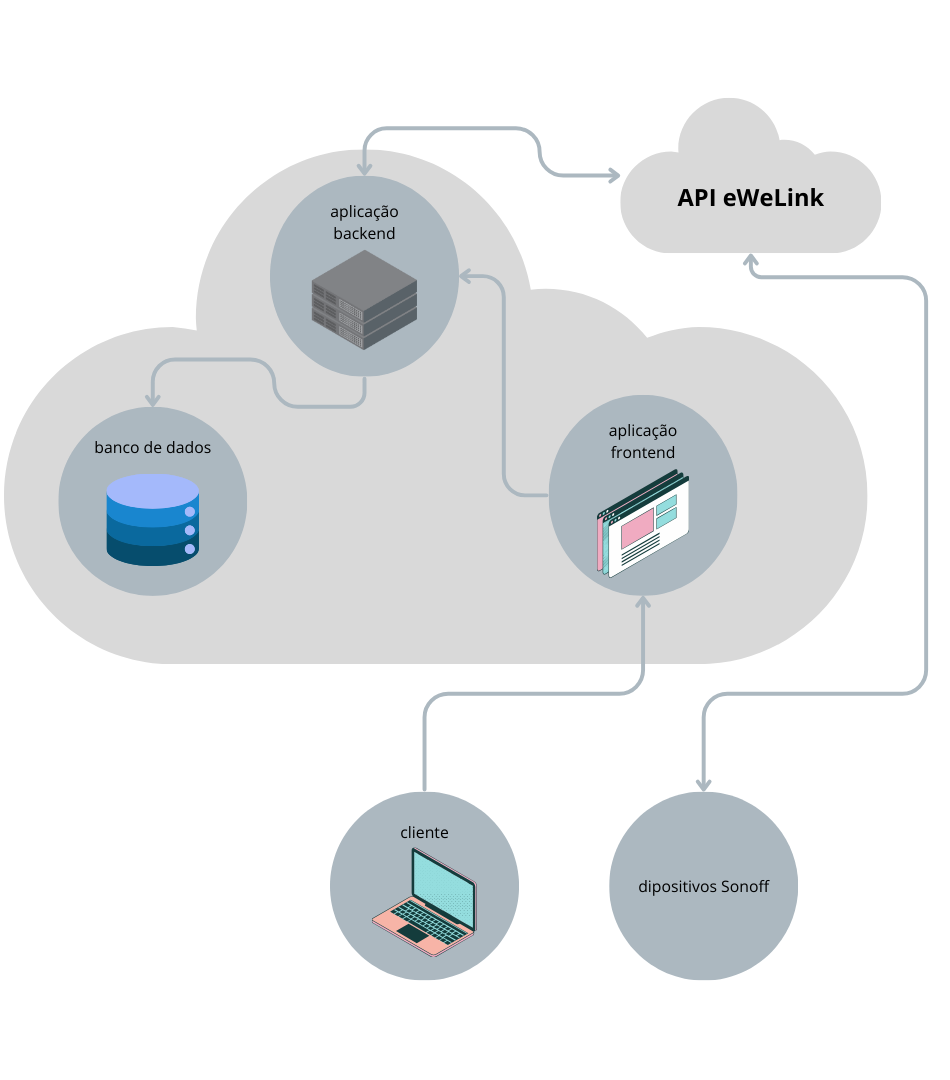
\includegraphics[scale=0.5]{images/cap4/arquitetura_geral.png}
	\end{center}
	\fonte{Autor.}
\end{figure}

O sistema adotará uma abordagem \textit{multi-tenant}, permitindo que múltiplas empresas utilizem a mesma plataforma de maneira independente. O administrador de cada empresa poderá configurar seu próprio ambiente, definindo nome, horários de funcionamento e quantidade de quadras disponíveis. Cada quadra terá horários de funcionamento ajustáveis de acordo com os dias da semana, garantindo flexibilidade na gestão.

Também foi considerada uma abordagem \textit{single-tenant} e replicável para cada cliente. O problema dessa abordagem é que a manutenção de cada instância do sistema seria mais custosa e complexa, pois cada cliente teria seu próprio banco de dados e instância do sistema. Além disso a necessidade de configuração manual para cada novo cliente seria trabalhosa e custosa para o time da Fischertec. A abordagem \textit{multi-tenant} é mais escalável e econômica, pois todos os clientes compartilham a mesma instância do sistema e banco de dados, com isolamento de dados e configurações.

Os clientes esportistas poderão acessar a plataforma para visualizar a disponibilidade das quadras de uma empresa em tempo real, selecionar um horário específico e realizar a reserva de forma simples e intuitiva. A confirmação das reservas será imediata por padrão, proporcionando uma experiência eficiente e conveniente tanto para os usuários quanto para os administradores. Será possível, também, configurar a necessidade de aprovação para as reservas, caso a empresa deseje revisar manualmente cada solicitação.

A fim de garantir a integração com dispositivos IoT de maneira simples e sem necessidade de conhecimento técnico por parte dos administradores das empresas, optou-se por utilizar uma solução de hardware consolidada no mercado, a Sonoff, que oferece dispositivos de automação residencial com suporte a integração via API. Dessa maneira, evita-se a necessidade de um hardware e uma aplicação extra que se conectaria ao servidor fazendo uma espécie de ponte para gerenciar os dispositivos IoT diretamente através da rede local. Além disso seria necessário uma configuração extra para liberar o controle local nos dispositivos Sonoff (o modo DIY \textit{Do It Yourself}) e atribuição de ips fixos na rede local (pois em caso de mudança de ip, seria necessário reconfigurar a aplicação de ponte para que ela pudesse encontrar os dispositivos na rede).

Portanto, a automação do controle dos dispositivos IoT será feita por meio da integração com a plataforma eWeLink da Shenzhen Coolkit Technology CO., LTD, amplamente utilizada no mercado e compatível com dispositivos da marca Sonoff. O administrador poderá conectar sua conta eWeLink ao sistema, permitindo a identificação automática dos dispositivos configurados. Esses dispositivos poderão ser atribuídos às quadras e configurados para executar comandos específicos no início e/ou fim de uma reserva, como ligar ou desligar iluminação e climatização de forma automatizada. Essa solução permitirá que os administradores da empresa configurem facilmente os dispositivos IoT para funcionarem em conjunto com a plataforma, sem a necessidade de contatar profissionais de tecnologia ou executar instruções complexas, reduzindo a abertura de chamados de suporte da aplicação.

Com essa abordagem, o sistema proporcionará um gerenciamento eficiente e automatizado das quadras esportivas, reduzindo desperdícios, otimizando recursos e melhorando a experiência dos clientes. Além disso, a solução contribuirá para a redução de custos operacionais e impacto ambiental, tornando-se uma ferramenta indispensável para empresas que buscam modernização e eficiência em sua gestão.

O desenvolvimento do sistema completo será dividido em duas etapas: backend e frontend. Neste projeto de fim de curso, será abordada a implementação do backend, que consiste na construção de uma aplicação de servidor responsável por toda a lógica de negócios e integração com a plataforma eWeLink. A aplicação será desenvolvida em Node.js, utilizando o framework Nest.js na linguagem Typescript, afim de satisfazer os requisitos técnicos apresentados. Terá suporte a cadastro, autenticação e autorização de usuários, persistência de dados em um banco de dados PostgreSQL e integração com a API da eWeLink.


% ---

% ---
% 5 - Capítulo 5
% ---
% ----------------------------------------------------------
\chapter{Desenvolvimento e Análise dos Resultados Obtidos}\label{cap:desenvolvimento_e_analise_resultados}
% ----------------------------------------------------------
Este capítulo apresenta o processo de desenvolvimento do sistema de gerenciamento de reservas e controle automatizado de dispositivos IoT para quadras esportivas. Na \autoref{sec:ferramentas_tecnologias} são apresentadas as ferramentas e tecnologias utilizadas no desenvolvimento do sistema. A \autoref{sec:desenvolvimento} apresenta o processo de desenvolvimento do PFC e a \autoref{sec:analise_resultados} dispõe dos resultados alcançados ao fim do processo.

% \textbf{Instruções da Coordenação do PFC:}

% Neste capítulo, deve-se:
% \begin{itemize}
% 	\item Descrever detalhadamente como foi feita a implementação/desenvolvimento da solução proposta;
% 	\item Deixar bem claro e justificar tecnicamente para o leitor como que o desenvolvimento realizado implementa de fato a solução proposta, explicando tecnicamente as decisões que foram tomadas para se chegar a tal implentação;
% 	\item Analisar os resultados obtidos com base em indicadores, gráficos, estatísticas, etc: 
% 	\begin{itemize}
% 		\item A implementação realizada solucionou de fato o problema tratado? 
% 		\item Obteve-se o resultado esperado? 
% 		\item Mostrou-se melhor que o método anterior?
% 		\item Vantagens e desvantagens; 
% 		\item Problemas encontrados;   
% 		\item Impacto dos resultados obtidos nos processos/projetos/produtos/serviços/clientes da empresa/instituto de pesquisa; 
% 		\item Impactos organizacionais, tecnológicos, financeiros, éticos, ecológicos, etc.
% 	\end{itemize}
% \end{itemize}

% Sugere-se colocar uma diagrama/fluxograma ilustrando como que a solução proposta foi implementada/desenvolvida, e depois explicar em detalhes cada parte/bloco do diagrama/fluxograma ao longo do texto. 

% Ressaltamos que, em princípio, existe uma infinidade de maneiras diferentes de implementar a solução proposta. Desse modo, o diagrama/fluxograma da solução proposta apresentado no capítulo anterior é mais geral e abstrato que o diagrama/fluxograma da implementação: a implementação realizada no PFC é uma maneira específica de se chegar à solução proposta a partir das técnicas, ferramentas e métodos utilizados. 

Alguns pontos que serão explicados nesse capítulo:

\begin{itemize}
	\item \textbf{Ferramentas}: As tecnologias utilizadas na implementação da solução proposta, como linguagens de programação, frameworks, bibliotecas, etc.
	\item \textbf{Arquitetura da solução}: A arquitetura utilizada na implementação da solução proposta, como monolítica, microsserviços, cliente-servidor, etc.
	\item \textbf{Modelagem do banco de dados}: O modelo utilizado para representar os dados da aplicação, incluindo as entidades, relacionamentos, atributos, etc.
	\item \textbf{\textit{backend}}: A parte da solução que lida com a manipulação dos dados e a regra de negócio da aplicação.
	\subitem{\textbf{Registro e autenticação de usuários}: Como o backend implementa a funcionalidade de registro e autenticação de usuários, incluindo validações, segurança, etc.}
	\subitem{\textbf{Autorização de usuários}: Como o \textit{backend} implementa a funcionalidade de autorização de usuários, incluindo permissões, roles, etc.}
	\subitem{\textbf{Rotas da aplicação}: Como o \textit{backend} implementa as rotas da aplicação, incluindo endpoints de CRUD para tenanants, quadras, agendamentos de horários e credenciais de acesso a API relacionada à internet das coisas (IoT).}
	\subitem{\textbf{Detalhamento do agendamentos de horários}: Como o \textit{backend} implementa a funcionalidade de agendamentos de horários de quadras, incluindo informações sobre os locais, os tipos de atividades, as datas e as horas.}
	\subitem{\textbf{Detalhamento da integração com IoT}: Como o \textit{backend} implementa a integração com dispositivos IoT e comanda o acionamento e desligamento de acordo com os agendamentos feitos pelosus usuários.}
	\item \textbf{Análise de resultados}: Análise dos resultados obtidos com o desenvolvimento da aplicação. Detalhando os principais aspesctos relevantes, como a eficiência do agendamento de horários, a segurança das informações e a integração com IoT.
\end{itemize}

\section{Ferramentas e Tecnologias Utilizadas}\label{sec:ferramentas_tecnologias}

A seção de ferramentas e tecnologias utilizadas no desenvolvimento deste projeto apresenta um panorama detalhado dos recursos técnicos empregados para a construção da aplicação de servidor do sistema de gerenciamento de reservas e controle automatizado de dispositivos IoT para quadras esportivas. 
% O projeto foi desenvolvido utilizando uma stack moderna e robusta, com o \textit{backend} implementado em Nest.js, um framework eficiente e escalável para Node.js, e o \textit{frontend} será desenvolvido em React, a fim de proporcionar uma experiência de usuário dinâmica e responsiva. Além disso, o banco de dados relacional PostgreSQL foi utilizado para garantir a integridade e a consistência dos dados, enquanto a integração com a plataforma eWeLink permitiu o controle automatizado de dispositivos IoT, agregando um nível adicional de automação e inovação ao sistema. Este conjunto de ferramentas foi escolhido com o objetivo de garantir um desenvolvimento ágil, eficiente e que atendesse às necessidades específicas do projeto.

\subsection{Git}

O Git é um sistema de controle de versão distribuído criado por Linus Torvalds em 2005, inicialmente para o desenvolvimento do kernel do Linux. Antes do Git, o projeto Linux utilizava o BitKeeper, mas devido a restrições de licenciamento, Torvalds decidiu desenvolver uma ferramenta própria. O objetivo principal era criar um sistema rápido, eficiente e que suportasse grandes projetos com facilidade.

As principais funções do Git incluem rastreamento de alterações no código-fonte, permitindo que múltiplos desenvolvedores trabalhem simultaneamente em um mesmo projeto sem conflitos. O Git possibilita a criação de ramificações (branches) para desenvolver novos recursos ou corrigir bugs de forma isolada, facilitando a integração dessas alterações ao projeto principal posteriormente. Além disso, como um sistema distribuído, cada desenvolvedor possui uma cópia completa do repositório, o que aumenta a segurança e a integridade dos dados. Atualmente, o Git é a ferramenta de controle de versão mais popular do mundo, amplamente utilizada por empresas de software, desenvolvedores independentes e projetos de código aberto.

Decidiu-se utilizar o Git devido a familiaridade da equipe com a ferramenta, já que é amplamente usada em outros projetos na empresa, além de sua robustez e confiabilidade.
 
O Git revolucionou a forma como o desenvolvimento de software é conduzido, proporcionando uma maneira eficiente e colaborativa de gerenciar projetos complexos. Sua flexibilidade, velocidade e robustez tornaram-no uma ferramenta essencial no arsenal de qualquer desenvolvedor, suportando desde pequenos projetos individuais até grandes sistemas empresariais.

\subsection{GitHub}

O GitHub é uma plataforma de hospedagem e repositório de código-fonte e arquivos que utiliza o Git para controle de versão. A plataforma permite que programadores ou qualquer usuário cadastrado contribuam em projetos, sejam eles privados ou de código aberto, de qualquer lugar do mundo. Amplamente adotada por desenvolvedores, o GitHub facilita a divulgação de trabalhos e a colaboração em projetos, além de oferecer recursos que simplificam a comunicação, como a identificação de problemas e a mesclagem de repositórios remotos por meio de issues e pull requests.

Atualmente, o GitHub é utilizado globalmente, contando com mais de 36 milhões de usuários ativos que contribuem em projetos comerciais ou pessoais. A plataforma hospeda mais de 100 milhões de projetos, incluindo alguns de renome mundial, como WordPress, GNU/Linux, Atom e Electron. Além disso, o GitHub oferece suporte a recursos de organização, amplamente utilizados por aqueles que desejam expandir seus projetos.

O Github é uma ferramenta usada por padrão na Fischertec. Embora outras plataformas como o Gitlab tenham funções semelhantes, optou-se por manter o padrão da empresa.

\subsection{PostgreSQL}

O \acrlong{SQL} foi desenvolvido nos anos 1970 pela IBM como uma linguagem padrão para gerenciar e manipular bancos de dados relacionais. PostgreSQL, um sistema de gerenciamento de banco de dados relacional, surgiu na Universidade da Califórnia em Berkeley, no final dos anos 1980, como parte do projeto POSTGRES (Post Ingres). Em 1996, o sistema foi renomeado para PostgreSQL, refletindo sua compatibilidade com SQL. Desde então, PostgreSQL evoluiu significativamente, tornando-se uma das bases de dados relacionais mais robustas e avançadas disponíveis.

PostgreSQL oferece uma ampla gama de funções, incluindo suporte a transações ACID (Atomicidade, Consistência, Isolamento, Durabilidade), integridade referencial, e extensões para manipulação de dados complexos como JSON e XML. Além disso, suporta procedimentos armazenados, gatilhos e uma variedade de tipos de índices para otimizar consultas. Atualmente, PostgreSQL é amplamente utilizado por grandes empresas, startups e projetos de código aberto devido à sua confiabilidade, flexibilidade e conformidade com os padrões SQL.

Existem outras soluções de banco de dados SQL como MySQL, que é conhecido por sua facilidade de uso e performance em aplicações web, e soluções NoSQL como MongoDB, que é ideal para armazenar grandes volumes de dados não estruturados e aplicações que exigem alta escalabilidade e flexibilidade. Optou-se por usar o PostgreSQL no desenvolvimento do projeto devido à sua capacidade de lidar com transações complexas, suporte a dados estruturados e não estruturados, e forte conformidade com os padrões SQL, o que garante integridade e consistência dos dados.

O PostgreSQL se destaca como uma solução de banco de dados robusta e versátil, adequada para uma ampla gama de aplicações. Sua evolução ao longo dos anos e a capacidade de suportar funcionalidades avançadas o tornam uma escolha excelente para projetos que exigem confiabilidade e flexibilidade. A decisão de utilizá-lo no projeto foi fundamentada em sua capacidade de atender às necessidades específicas de gerenciamento de dados de maneira eficiente e segura.

\subsection{Typescript}

O JavaScript, criado em 1995 por Brendan Eich da Netscape, rapidamente se tornou a linguagem padrão para desenvolvimento web, permitindo a criação de páginas dinâmicas e interativas. No entanto, à medida que aplicações web se tornavam mais complexas, as limitações de JavaScript em termos de tipagem estática e suporte para grandes projetos se tornaram evidentes. Para reduzir essas limitações, a Microsoft lançou o TypeScript em 2012, uma linguagem de programação de código aberto que é um superconjunto (superset) estrito de JavaScript. TypeScript adiciona tipagem estática e outros recursos avançados ao JavaScript, ajudando os desenvolvedores a escrever código mais seguro e escalável.

As principais funções do TypeScript incluem a adição de tipos estáticos, interfaces, classes e módulos, que não existem nativamente no JavaScript. Essas funcionalidades permitem a detecção de erros durante o desenvolvimento, antes do tempo de execução, melhorando a qualidade do código. Além disso, TypeScript se transpila (é convertido) para JavaScript, garantindo compatibilidade total com os navegadores e plataformas que suportam JavaScript. Atualmente, TypeScript é amplamente adotado em projetos de grande escala devido à sua capacidade de melhorar a produtividade e a manutenção do código. Empresas como Google, Microsoft e Airbnb utilizam TypeScript em seus projetos.

No desenvolvimento do projeto \textit{backend}, optou-se por TypeScript em vez de JavaScript por várias razões. TypeScript proporciona uma melhor experiência de desenvolvimento, oferecendo autocompletar, navegação de código e verificação de tipos em tempo de compilação, o que ajuda a evitar muitos erros comuns em JavaScript. Isso é especialmente importante em projetos \textit{backend}, onde a robustez e a previsibilidade do código são cruciais. Além disso, TypeScript facilita a colaboração entre desenvolvedores, permitindo que eles entendam e mantenham o código com mais facilidade.

O TypeScript se destaca como uma ferramenta poderosa que complementa e aprimora JavaScript, tornando o desenvolvimento de software mais eficiente e menos propenso a erros. Sua adoção no desenvolvimento da aplicação \textit{backend} de gerenciamento de reservas e controle automatizado de dispositivos IoT permitiu criar um código mais robusto e sustentável.

\subsection{Node.js}

O Node.js é uma plataforma de desenvolvimento open-source baseada no motor JavaScript V8 do Google Chrome, criada em 2009 por Ryan Dahl. Seu objetivo inicial era possibilitar a execução de JavaScript no lado do servidor, permitindo o desenvolvimento de aplicações web com maior eficiência e escalabilidade. Desde seu lançamento, o Node.js rapidamente ganhou popularidade devido à sua arquitetura orientada a eventos e sua capacidade de lidar com operações de entrada e saída de forma não bloqueante, o que é particularmente útil para aplicações em tempo real.

Atualmente, o Node.js é amplamente utilizado para construir desde APIs e microservices até aplicações completas de grande escala. Sua capacidade de executar JavaScript tanto no cliente quanto no servidor facilita o desenvolvimento fullstack, enquanto a vasta biblioteca de pacotes disponíveis através do npm (Node Package Manager) oferece soluções para praticamente qualquer necessidade de desenvolvimento. O Node.js tem sido uma escolha popular em diversas indústrias devido à sua performance, escalabilidade e ao suporte contínuo de uma grande comunidade de desenvolvedores.

Uma das principais vantagens do Node.js em comparação com outras soluções é sua natureza assíncrona e orientada a eventos, que permite o gerenciamento eficiente de múltiplas conexões simultâneas sem sobrecarregar os recursos do servidor. Além disso, a utilização de JavaScript, uma linguagem amplamente conhecida e utilizada, reduz a curva de aprendizado para novos desenvolvedores e facilita a integração entre equipes de \textit{frontend} e \textit{backend}. A modularidade do Node.js e sua grande comunidade de apoio também contribuem para o desenvolvimento mais rápido e eficiente de aplicações.

Portanto o Node.js se destaca como uma solução versátil e eficiente para o desenvolvimento de aplicações modernas. Sua combinação de performance, escalabilidade e uma vasta gama de ferramentas e bibliotecas tornam-no uma escolha robusta para desenvolvedores que buscam criar aplicações rápidas e escaláveis, atendendo às demandas de um mercado cada vez mais dinâmico e competitivo.

\subsection{Nest.js}

O Nest.js é um framework de desenvolvimento \textit{backend} criado em 2017 por Kamil Myśliwiec. Inspirado nos princípios de programação modular e fortemente influenciado pelo Angular, o Nest.js foi projetado para oferecer uma estrutura robusta e escalável para a construção de aplicações do lado do servidor. Desde o seu lançamento, o framework tem crescido em popularidade, especialmente entre desenvolvedores que buscam uma abordagem moderna para o desenvolvimento de aplicações \textit{backend} em Node.js.

O Nest.js fornece uma arquitetura modular que facilita a criação e a manutenção de aplicações escaláveis e bem estruturadas. Ele suporta diversos paradigmas de programação, incluindo orientação a objetos, programação funcional e reativa. Com suporte nativo para TypeScript, o Nest.js oferece tipagem estática, o que melhora a confiabilidade e a legibilidade do código. Atualmente, é amplamente utilizado para construir APIs RESTful, microservices e aplicativos monolíticos, sendo uma escolha frequente em projetos que exigem alta escalabilidade e flexibilidade.

Entre as principais vantagens do Nest.js estão sua modularidade, que permite a criação de aplicações altamente organizadas e de fácil manutenção, e seu suporte integral a TypeScript, que traz maior segurança e produtividade no desenvolvimento. Em comparação com outros frameworks, como Express.js, o Nest.js oferece uma estrutura mais robusta e orientada a boas práticas, facilitando o desenvolvimento de aplicações complexas. No contexto do \acrlong{PFC}, o Nest.js foi escolhido por sua capacidade de suportar a criação de uma aplicação \textit{multi-tenant} complexa, com necessidades específicas de escalabilidade, organização e integração com outras tecnologias.

O Nest.js se destaca como uma ferramenta poderosa para o desenvolvimento de aplicações \textit{backend} modernas, combinando a performance do Node.js com uma arquitetura flexível e escalável. Sua adoção neste \acrlong{PFC} reflete a busca por soluções eficientes e de alta qualidade, alinhadas com as demandas atuais do mercado de tecnologia.

\subsection{Docker}

O Docker foi lançado em 2013 por Solomon Hykes, inicialmente como um projeto interno da empresa dotCloud. A plataforma foi criada com o objetivo de simplificar o processo de desenvolvimento, distribuição e execução de aplicações por meio da virtualização de contêineres. Desde seu lançamento, o Docker tem revolucionado a maneira como aplicações são desenvolvidas e implantadas, tornando-se uma das ferramentas mais populares no ecossistema de DevOps.

Atualmente, o Docker é amplamente utilizado para criar, distribuir e executar aplicações em contêineres, que são ambientes leves e portáteis que contêm tudo o que uma aplicação precisa para ser executada. Isso inclui código, bibliotecas e dependências, garantindo que a aplicação funcione de maneira consistente em qualquer ambiente. O Docker é uma escolha comum em projetos que exigem portabilidade, escalabilidade e uma integração contínua eficiente, sendo adotado por empresas de todos os tamanhos para modernizar seus fluxos de trabalho de desenvolvimento e implantação.

Entre as principais vantagens do Docker estão a portabilidade de aplicações, a eficiência no uso de recursos e a facilidade de integração com pipelines de CI/CD (integração contínua e entrega contínua). Comparado com máquinas virtuais tradicionais, os contêineres do Docker são mais leves e rápidos, o que resulta em tempos de inicialização menores e melhor utilização de recursos. No contexto deste projeto, o Docker foi escolhido para garantir que o ambiente de desenvolvimento e produção seja consistente, facilitando a implantação em servidores AWS e reduzindo problemas de compatibilidade.

O Docker se destaca como uma solução essencial para o desenvolvimento e a implantação de aplicações modernas, oferecendo uma maneira eficiente de gerenciar ambientes de software. Sua escolha neste projeto reflete a busca por uma solução que ofereça portabilidade, eficiência e flexibilidade, alinhando-se às melhores práticas do mercado e garantindo um processo de desenvolvimento mais ágil e confiável.

\subsection{Postman}

O Postman foi lançado em 2012 por Abhinav Asthana como uma ferramenta auxiliar para o desenvolvimento de APIs. Inicialmente criado como uma extensão para o Google Chrome, o Postman rapidamente evoluiu para uma aplicação completa e independente, tornando-se uma das ferramentas mais populares para o teste e desenvolvimento de APIs. Ao longo dos anos, a plataforma expandiu suas funcionalidades para atender às crescentes demandas de desenvolvedores e equipes de API.

O Postman é amplamente utilizado para testar, documentar e monitorar APIs, oferecendo uma interface amigável que facilita a realização de requisições HTTP, o gerenciamento de coleções de APIs e a automatização de testes. Além disso, ele permite a colaboração em equipe, possibilitando o compartilhamento de coleções e ambientes de teste. Atualmente, o Postman é uma ferramenta indispensável no fluxo de trabalho de desenvolvedores e engenheiros de qualidade, sendo utilizado por milhões de usuários ao redor do mundo.

As vantagens do Postman incluem sua interface intuitiva, que reduz a complexidade do teste de APIs, e suas capacidades avançadas de automação e documentação. Comparado a outras ferramentas, como cURL ou alternativas mais básicas, o Postman oferece uma experiência mais integrada e acessível, especialmente para equipes que precisam colaborar em projetos complexos. No desenvolvimento deste projeto, o Postman foi escolhido por sua facilidade de uso e suas capacidades de automação de testes, o que contribui para um processo de desenvolvimento mais eficiente e menos propenso a erros.

Portanto o Postman se consolida como uma ferramenta essencial para o desenvolvimento e manutenção de APIs, oferecendo funcionalidades abrangentes que facilitam o trabalho de desenvolvedores e equipes de qualidade. Sua utilização neste projeto destaca a importância de ferramentas que otimizam o fluxo de trabalho, garantindo maior eficiência e qualidade no desenvolvimento de sistemas modernos.


\section{Desenvolvimento}\label{sec:desenvolvimento}

Após apresentadas as ferramentas e tecnologias selecionadas na \autoref{sec:ferramentas_tecnologias}, esta seção tratará do desenvolvimento do projeto \textit{backend} da aplicação.

\subsection{Configuração Inicial do Projeto}\label{subsec:configuracao_inicial}

A primeira etapa do projeto se deu pela configuração do ambiente de desenvolvimento. Para isso, foi o inicializado um novo projeto Nest.js com os comandos

\begin{verbatim}
	nest new sports
\end{verbatim}
e instaladas as dependências necessárias. Algumas das bibliotecas usadas estão listadas na \autoref{tab:bibliotecas}.

\begin{table}[htb]
	\centering
	\caption{\label{tab:bibliotecas}Bibliotecas utilizadas.}	
	\begin{tabular}{|l|p{4cm}|}
		\hline
		\textbf{Nome} & \textbf{versão} \\ \hline
    \text{@nestjs/cache-manager} & 2.0.1 \\ \hline
    \text{@nestjs/common} & 10.0.0 \\ \hline
    \text{@nestjs/jwt} & 10.1.0 \\ \hline
    \text{@nestjs/platform-express} & 10.0.0 \\ \hline
    \text{@nestjs/schedule} & 4.1.2 \\ \hline
    \text{@nestjs/typeorm} & 10.0.0 \\ \hline
    \text{bcrypt} & 5.1.1 \\ \hline
    \text{class-transformer} & 0.5.1 \\ \hline
    \text{class-validator} & 0.14.0 \\ \hline
    \text{colors} & 1.4.0 \\ \hline
    \text{dotenv} & 16.0.3 \\ \hline
    \text{ewelink-api-next} & 1.0.4 \\ \hline
    \text{moment} & 2.30.1 \\ \hline
    \text{pg} & 8.11.3 \\ \hline
    \text{reflect-metadata} & 0.1.13 \\ \hline
    \text{rxjs} & 7.8.1 \\ \hline
    \text{typeorm} & 0.3.17 \\ \hline
    \text{uuid} & 9.0.1 \\ \hline
	\end{tabular}
	\fonte{Autor.}
\end{table}

Em seguida os cointêneres Docker foram configurados para executar o banco de dados PostgreSQL e o PgAdmin (Interface Gráfica para gerenciar o banco de dados PostgreSQL) através de um arquivo docker-compose. Com o ambiente de desenvolvimento configurado, foi realizada a configuração da conexão da aplicação com o banco de dados PostgreSQL com auxílio da biblioteca TypeOrm. O TypeORM é uma biblioteca ORM (Object-Relational Mapping) para TypeScript e JavaScript, que facilita a interação com bancos de dados relacionais. Ele permite a abstração do banco de dados, permitindo que os desenvolvedores se concentrem na manipulação dos dados em vez da implementação detalhada das operações SQL.

\subsection{Arquitetura de Pastas}\label{subsec:arquitetura_pastas}

A arquitetura do projeto foi dividida em pastas para organizar o código fonte e facilitar a manutenção, seguindo a metodologia de arquitetura modular e de camadas. A pasta "src" contém todos os arquivos do projeto, divididos em pastas para cada funcionalidade ou recurso do sistema. As principais pastas são "config" (configuração do TypeORM com PostgreSQL) , "db" (configuração da conexão do banco PostgreSQL), "modules" (módulos dos recursos da aplicação, como \textit{tenants}, \textit{users} e etc.) e "resources" (como funções de manipulação de dados, \textit{pipes} para criptografia de senhas, \textit{interceptors} para logs de informações e \textit{filters} para tratamento de erros). A arquitetura de pastas está exemplificada na \autoref{fig:arquitetura_pastas}

\begin{figure}[htp]
	\caption{\label{fig:arquitetura_pastas}Arquitetura de pastas da aplicação \textit{backend}.}
	\begin{center}
	  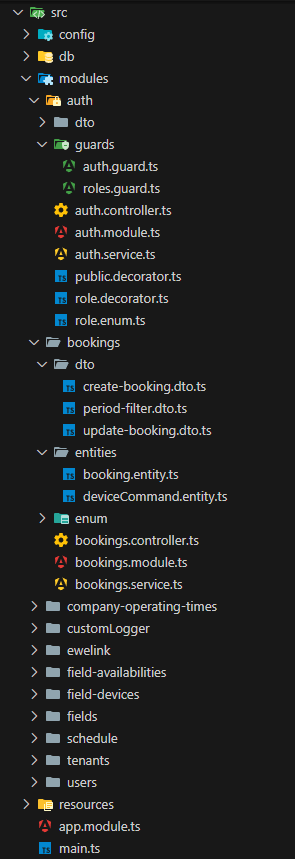
\includegraphics[scale=0.5]{images/cap5/arq_pastas.png}
	\end{center}
	\fonte{Autor.}
\end{figure}

\subsection{Implementação das Funcionalidades}\label{subsec:implementacao_funcionalidades}

Nessa seção serão detalhadas as implementações das funcionalidades do sistema. Serão abordados o modelo de dados em \ref{subsubsec:modelagem_banco_dados}, autenticação e autorização em \ref{subsubsec:autenticacao_autorizacao}, \textit{tenants} em \ref{subsubsec:modulo_tenants}, módulos de usuários em \ref{subsubsec:modulo_usuarios}, quadras e disponibilidade de quadras em \ref{subsubsec:modulos_quadras_disponibilidade_quadras}, integração com a API eWeLink em \ref{subsubsec:integacao_ewelink}, quadras-dispositivos em \ref{subsubsec:modulo_quadras_dispositivos}, reservas e comandos IoT em \ref{subsubsec:modulo_reservas} e o envio de comandos aos dispositivos IoT em \ref{subsubsec:envio_comandos_iot}. Algumas rotas e implementações serão mostradas e detalhadas como exemplo e outras ocultadas a fim de reduzir a extensão do texto.

\subsubsection{Modelagem do Banco de Dados}\label{subsubsec:modelagem_banco_dados}
A primeira etapa do desenvolvimento do sistema é a modelagem do banco de dados. Nesta etapa, são criados os diagramas entidade-relacionamento (ER) que representam as entidades e seus relacionamentos. O diagrama ER é uma representação visual das tabelas do banco de dados e dos relacionamentos entre elas e está apresentado na \autoref{fig:modelagem_banco_dados}.

\begin{figure}[htp]
	\caption{\label{fig:modelagem_banco_dados}Modelagem do Banco de Dados.}
	\begin{center}
	  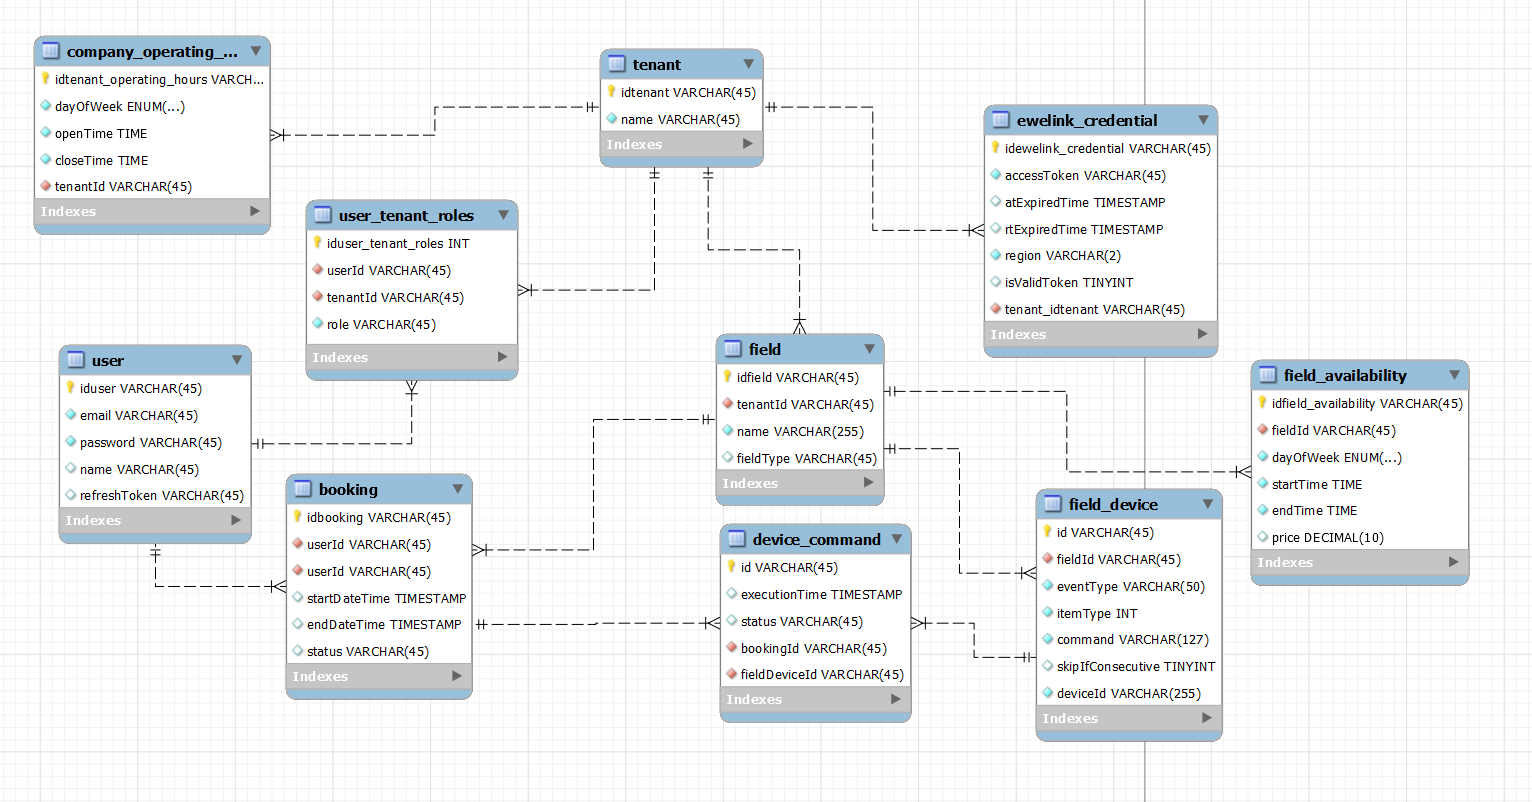
\includegraphics[scale=0.38]{images/cap5/modelage_banco_dados.png}
	\end{center}
	\fonte{Autor.}
\end{figure}

\noindent\textbf{\textit{tenant} (Locatário/Empresa)}\\
Armazena informações das empresas que utilizam o sistema. Cada empresa tem um ambiente isolado para suas configurações e dados.\\
Relacionamentos:
\begin{itemize}
	\item Relaciona-se com \texttt{field} (uma empresa pode ter várias quadras).
	\item Relaciona-se com \texttt{user\_tenant\_roles} (definição de papéis dos usuários dentro da empresa).
	\item Relaciona-se com \texttt{ewelink\_credential} (armazenamento de credenciais IoT por empresa).
	\item Relaciona-se com \texttt{company\_operating\_hours} (definição do horário de funcionamento da empresa).
\end{itemize}

\noindent\textbf{\textit{user} (Usuário do Sistema)}\\
Cadastra usuários na plataforma, permitindo o acesso e gestão de informações dos usuários em diferentes locatários. \\
Relacionamentos: 
\begin{itemize} 
	\item Relaciona-se com \texttt{use\_tenant\_roles} (um usuário pode ter diferentes papéis em empresas distintas). 
	\item Relaciona-se com \texttt{booking} (usuários realizam reservas de quadras). 
\end{itemize}

\noindent\textbf{\textit{user\textunderscore tenant\textunderscore roles} (Papéis de Usuário na Empresa)}\\
Define os papéis dos usuários em diferentes locatários, garantindo acesso e permissões personalizadas para cada perfil. \\
Relacionamentos: 

\begin{itemize} 
	\item Relaciona-se com \texttt{user} (indica o usuário). 
	\item Relaciona-se com \texttt{tenant} (indica a empresa onde o usuário tem um papel). 
\end{itemize}


\noindent\textbf{\textit{company\textunderscore operating\textunderscore hours} (Horários de Funcionamento da Empresa)}\\
Define os horários de funcionamento das empresas, permitindo customização e gestão do tempo disponível para operações em cada locatário. \\
Relacionamentos: 

\begin{itemize} 
	\item Relaciona-se com \texttt{tenant} (cada locatário tem seus próprios horários de funcionamento). 
\end{itemize}


\noindent\textbf{\textit{field} (Quadras Esportivas)}\\
Armazena as quadras disponíveis para reservas, relacionadas ao locatário que as possui e contendo informações específicas sobre cada quadra. \\
Relacionamentos: 

\begin{itemize} 
	\item Relaciona-se com \texttt{tenant} (cada locatário pode ter várias quadras). 
	\item Relaciona-se com \texttt{field\_availability} (definição de horários disponíveis para a quadra). 
	\item Relaciona-se com \texttt{field\_device} (dispositivos IoT associados à quadra). 
	\item Relaciona-se com \texttt{booking} (quadras podem ser reservadas). 
\end{itemize}


\noindent\textbf{\textit{field\textunderscore availability} (Disponibilidade da Quadra)}\\
Determina os horários disponíveis para cada quadra, indicando o período de tempo em que a mesma fica aberta e quanto custa o uso dela. \\
Relacionamentos: 

\begin{itemize} 
	\item Relaciona-se com \texttt{field} (define a disponibilidade para cada quadra). 
\end{itemize}


\noindent\textbf{\textit{booking} (Reservas de Quadras)}\\
Registra as reservas feitas pelos usuários, associando-as ao locatário que possui a quadra reservada e outros detalhes sobre o horário, usuário e status da reserva. \\
Relacionamentos: 

\begin{itemize} 
	\item Relaciona-se com \texttt{user} (quem fez a reserva). 
	\item Relaciona-se com \texttt{field} (qual quadra foi reservada). 
\end{itemize}


\noindent\textbf{\textit{ewelink\textunderscore credentia}l (Credenciais para Controle IoT via eWeLink)}\\
Armazena informações de autenticação da integração entre o sistema e dispositivos IoT, como tokens de acesso e gerenciamento de recursos. \\
Relacionamentos: 

\begin{itemize} 
	\item Relaciona-se com \texttt{tenant} (cada locatário pode ter credenciais IoT). 
\end{itemize}


\noindent\textbf{\textit{field\textunderscore device} (Dispositivos IoT Associados às Quadras)}\\
Registra os dispositivos IoT instalados em cada quadra, indicando seu tipo de funcionalidade, comando a ser executado e outros detalhes relevantes para o gerenciamento. \\
Relacionamentos: 

\begin{itemize} 
	\item Relaciona-se com \texttt{field} (cada quadra pode ter vários dispositivos IoT). 
\end{itemize}


\noindent\textbf{\textit{device\textunderscore command} (Comandos Enviados a Dispositivos IoT)}\\
Armazena os comandos programados ou executados para dispositivos IoT, associados às reservas e que devem ser executados conforme a agenda de reservas. \\
Relacionamentos: 

\begin{itemize} 
	\item Relaciona-se com \texttt{booking} (comandos são acionados conforme reservas). 
	\item Relaciona-se com \texttt{field\_device} (cada comando pertence a um dispositivo IoT). 
\end{itemize}

\subsubsection{Autenticação e Autorização}\label{subsubsec:autenticacao_autorizacao}

\noindent\textbf{Visão Geral}\\
O módulo de autenticação é responsável por garantir a segurança e o controle de acesso ao sistema multi-tenant. Ele permite que os usuários se autentiquem utilizando credenciais seguras e fornece mecanismos para gerenciamento de tokens de acesso e renovação de sessão. O sistema utiliza autenticação baseada em tokens JWT (\textit{JSON Web Token}) e cookies para armazenar \textit{refresh tokens} com segurança.

A autenticação dos usuários é fundamental para garantir que apenas indivíduos autorizados tenham acesso aos recursos do sistema. Além disso, o módulo gerencia o login, o registro de novos usuários (inicialmente sem vínculo com nenhum \textit{tenant}), a renovação de tokens e o logout seguro, invalidando tokens de sessão comprometidos.

\noindent\textbf{Fluxo das Rotas}\\
O controlador de autenticação (\texttt{auth.controller.ts}) define os endpoints responsáveis pelo login, registro de novos usuários, renovação de tokens e logout. Ele interage com o serviço de autenticação (\texttt{auth.service.ts}), que contém a lógica de geração e validação de tokens, verificação de credenciais e manipulação segura de sessões.

\subsubsubsection{Autenticação de Usuário}
\begin{itemize}
	\item \textbf{Rota:} \texttt{POST /auth/login}
	\item \textbf{Descrição:} Permite que um usuário se autentique utilizando seu e-mail e senha. Retorna um \textit{access token} e um \textit{refresh token}.
	\item \textbf{Fluxo:}
	\begin{enumerate}
		\item O controlador recebe as credenciais do usuário.
		\item O serviço de autenticação busca o usuário no banco de dados e valida a senha.
		\item Se as credenciais forem válidas, um novo \textit{access token} e um \textit{refresh token} são gerados e retornados.
	\end{enumerate}
\end{itemize}

O código construído para o \textit{controller} e  o \textit{service} estão disponíveis no \autoref{cod:login-controller} e  no \autoref{cod:login-service}, respectivamente, e servirão de exemplo para os demais \textit{controllers} e \textit{services}.

\begin{lstlisting}[caption={Exemplo de \textit{controller} para \textit{login}.},label={cod:login-controller}]
	@Post('login')
  async login(
    @Res({ passthrough: true }) res: Response,
    @Body() { email, password }: AuthenticateDto
  ) {
    const { loggedUser, accessToken, refreshToken } =
      await this.authService.login(email, password)

    res.cookie('jwt', refreshToken, {
      httpOnly: true,
      sameSite: 'none',
      secure: true,
      maxAge: 24 * 60 * 60 * 1000
    })
    res.status(201)
    return { accessToken, ...loggedUser }
  }
\end{lstlisting}

\begin{lstlisting}[caption={Exemplo de \textit{service} para \textit{login}.},label={cod:login-service}]
	async login(email: string, insertedPassword: string) {
    try {
      const foundUser = await this.userService.searchForEmail(email)

      const userWasAuthenticated = await bcrypt.compare(
        insertedPassword,
        foundUser.password
      )

      if (!userWasAuthenticated)
        throw new UnauthorizedException('E-mail e/ou senha incorretos.')

      const payload: UserPayload = {
        sub: foundUser.id,
        email: foundUser.email,
        name: foundUser.name
      }

      const newRefreshToken = await this.createRefreshToken(payload)
      const newAccessToken = await this.createAccessToken(payload)

      await this.updateRefreshToken(newRefreshToken, {
        sub: foundUser.id,
        ...foundUser
      })

      return {
        accessToken: newAccessToken,
        refreshToken: newRefreshToken,
        loggedUser: payload
      }
    } catch (e) {
      if (e?.status === 404 || e?.status === 401)
        throw new UnauthorizedException('E-mail e/ou senha incorretos.')

      console.log('Erro interno:', e)
      throw new InternalServerErrorException(
        'Erro interno no servidor. ' + e?.message
      )
    }
  }
\end{lstlisting}

\subsubsubsection{Registro de Usuário}
\begin{itemize}
	\item \textbf{Rota:} \texttt{POST /auth/register}
	\item \textbf{Descrição:} Permite criar um novo usuário no sistema sem vinculação com nenhuma empresa, armazenando suas credenciais de forma segura.
	\item \textbf{Fluxo:}
	\begin{enumerate}
		\item O controlador recebe os dados do novo usuário.
		\item A senha é criptografada antes de ser salva no banco de dados.
		\item O usuário é criado e retornado na resposta.
	\end{enumerate}
\end{itemize}

\subsubsubsection{Renovação de Token}
\begin{itemize}
	\item \textbf{Rota:} \texttt{GET /auth/refresh}
	\item \textbf{Descrição:} Permite gerar um novo \textit{access token} utilizando um \textit{refresh token} válido armazenado em um cookie.
	\item \textbf{Fluxo:}
	\begin{enumerate}
		\item O controlador verifica a presença do \textit{refresh token} nos cookies da requisição.
		\item O serviço valida o token e gera um novo \textit{access token}.
		\item O novo token é retornado na resposta.
	\end{enumerate}
\end{itemize}

\subsubsubsection{Logout}
\begin{itemize}
	\item \textbf{Rota:} \texttt{GET /auth/logout}
	\item \textbf{Descrição:} Invalida a sessão do usuário removendo seu \textit{refresh token} armazenado.
	\item \textbf{Fluxo:}
	\begin{enumerate}
		\item O controlador verifica o \textit{refresh token} armazenado no cookie da requisição.
		\item O serviço de autenticação invalida o token no banco de dados.
		\item O cookie é removido da resposta e a sessão é encerrada.
	\end{enumerate}
\end{itemize}

\subsubsection{Módulo de Tenants}\label{subsubsec:modulo_tenants}

\noindent\textbf{Visão Geral} \\
O módulo de \textit{tenants} é responsável por gerenciar múltiplos locatários dentro do sistema, permitindo a criação, consulta, atualização e remoção de \textit{tenants}. Esse módulo é essencial para suportar um ambiente multi-tenant, onde cada empresa ou cliente pode operar de forma isolada dentro da mesma aplicação.

As principais funcionalidades deste módulo incluem:

\begin{itemize}
    \item Criação de um \textit{tenant}, associando-o a um usuário administrador.
    \item Consulta de \textit{tenants}, tanto de forma individual quanto em lista.
    \item Atualização das informações de um \textit{tenant}.
    \item Remoção de um \textit{tenant}.
    \item Controle de permissões para diferentes níveis de usuário dentro de um \textit{tenant}.
\end{itemize}

O acesso às rotas do módulo é protegido por um sistema de autenticação e autorização baseado em \textit{roles}, garantindo que apenas usuários autorizados possam executar determinadas ações.

\noindent\textbf{Fluxo das Rotas} \\
As rotas do módulo de \textit{tenants} são definidas no \texttt{TenantsController}, garantindo a estruturação adequada dos endpoints da API. A seguir, estão dispostos os fluxos de duas das principais operações: criação e busca de \textit{tenants}.

\subsubsubsection{Criação de um\textit{Tenant}}
\begin{itemize}
	\item \textbf{Rota:} \texttt{POST /tenants}
	\item \textbf{Descrição:} Criação de um novo \textit{tenant}.
	\item \textbf{Fluxo:}
	\begin{enumerate}
    \item O usuário autenticado envia uma requisição contendo os dados do novo \textit{tenant}.
    \item O serviço verifica se o usuário tem permissão para criar um \textit{tenant}.
    \item Se autorizado, os dados do \textit{tenant} são persistidos no banco de dados.
    \item O usuário criador recebe automaticamente o papel de administrador dentro do novo \textit{tenant}.
    \item A resposta retorna uma mensagem de sucesso e os detalhes do \textit{tenant} criado.
	\end{enumerate}
\end{itemize}

\subsubsubsection{Consulta de um\textit{Tenant}}
\begin{itemize}
	\item \textbf{Rota:} \texttt{GET /tenants/:id}
	\item \textbf{Descrição:} Buscar um \textit{tenant} específico.
	\item \textbf{Fluxo:}
	\begin{enumerate}
    \item O usuário faz uma requisição com o identificador do \textit{tenant} desejado.
    \item O serviço consulta o banco de dados para localizar o \textit{tenant} correspondente.
    \item Se encontrado, os detalhes do \textit{tenant} são retornados na resposta.
    \item Se o \textit{tenant} não for encontrado, uma exceção é lançada informando o erro.
	\end{enumerate}
\end{itemize}

\noindent\textbf{Outras Operações} \\
Além das rotas descritas acima, o módulo também disponibiliza endpoints para listar todos os \textit{tenants}, atualizar informações e remover um \textit{tenant}. Estas operações são protegidas por um sistema de autenticação e autorização baseado em \textit{roles}, garantindo que apenas usuários com as permissões adequadas possam realizá-las.

\subsubsection{Módulo de Usuarios}\label{subsubsec:modulo_usuarios}

\noindent\textbf{Visão Geral}\\
O módulo de usuários é responsável por gerenciar os perfis de usuários dentro do sistema multi-tenant. Ele permite o cadastro, consulta, edição e remoção de usuários (vinculados a uma empresa específica), além de possibilitar a gestão de papéis dentro de diferentes empresas. O sistema suporta diferentes níveis de acesso e autenticação baseada em tokens.

Os usuários podem pertencer a múltiplas empresas e ter diferentes papéis em cada uma delas. Isso permite um controle granular das permissões e acesso às funcionalidades do sistema.

\noindent\textbf{Fluxo das Rotas}\\
O controlador de usuários (\texttt{users.controller.ts}) define os endpoints para interação com o serviço de usuários (\texttt{users.service.ts}), que contém a lógica de negócio. O código construído para o \textit{controller} e  o \textit{service} estão disponíveis no \autoref{cod:create-user-controller} e  no \autoref{cod:create-user-service}, respectivamente, e servirão de exemplo para os demais \textit{controllers} e \textit{services}.

\subsubsubsection{Criação de Usuário}
\begin{itemize}
	\item \textbf{Rota:} \texttt{POST /tenant/:tenantId/users}
	\item \textbf{Descrição:} Permite criar um novo usuário, recebendo os dados básicos no corpo da requisição. Caso seja informado um \texttt{tenantId}, o usuário é vinculado a essa empresa.
	\item \textbf{Fluxo:}
	\begin{enumerate}
		\item O controlador recebe os dados do novo usuário.
		\item O serviço cria a entidade e a salva no banco.
		\item O usuário é retornado na resposta.
	\end{enumerate}
\end{itemize}

\begin{lstlisting}[caption={Exemplo de \textit{controller} para criação de usuário.},label={cod:create-user-controller}]
	@Post()
  async createUser(
    @Body() { password, ...userData }: CreateUserDTO,
    @Body('password', HashingPasswordPipe) hashedPassword: string
  ) {
    const createdUser = await this.userService.createUser({
      ...userData,
      password: hashedPassword
    })

    return {
      message: 'Usuario criado!',
      user: new ListUserDTO({ id: createdUser.id, name: createdUser.name })
    }
  }
\end{lstlisting}

\begin{lstlisting}[caption={Exemplo de \textit{service} para criação de usuário.},label={cod:create-user-service}]
	async createUser(userData: CreateUserDTO, tenantId?: string) {
    const userEntity = new User()

    Object.assign(userEntity, userData as User)
    const createdUser = await this.userRepository.save(userEntity)

    console.log('Create relation to tenant: ', tenantId)

    return createdUser
  }
\end{lstlisting}

\subsubsubsection{Consulta de Usuário por ID}
\begin{itemize}
	\item \textbf{Rota:} \texttt{GET /tenant/:tenantId/users/:id}
	\item \textbf{Descrição:} Retorna as informações detalhadas de um usuário, incluindo seus papéis nas empresas.
	\item \textbf{Fluxo:}
	\begin{enumerate}
		\item O controlador recebe o \texttt{id} do usuário via parâmetro de rota.
		\item O serviço busca o usuário no banco, carregando as relações necessárias.
		\item Caso não seja encontrado, retorna erro.
		\item Se encontrado, retorna os dados do usuário.
	\end{enumerate}
\end{itemize}

\subsubsubsection{Listagem de Usuários de uma Empresa}
\begin{itemize}
	\item \textbf{Rota:} \texttt{GET /tenant/:tenantId/users}
	\item \textbf{Descrição:} Retorna uma lista de usuários vinculados a uma empresa.
	\item \textbf{Fluxo:}
	\begin{enumerate}
		\item O controlador recebe o \texttt{tenantId} como um parâmetro.
		\item O serviço busca os usuários que possuem relação com essa empresa.
		\item Retorna a lista formatada.
	\end{enumerate}
\end{itemize}

\subsubsubsection{Atualização de Usuário}
\begin{itemize}
  \item \textbf{Rota:} \texttt{PATCH /tenant/:tenantId/users/:id}
  \item \textbf{Descrição:} Permite a edição dos dados cadastrais de um usuário.
  \item \textbf{Fluxo:}
  \begin{enumerate}
    \item O controlador recebe o \texttt{id} e os novos dados do usuário.
    \item O serviço verifica se o usuário existe.
    \item Caso não exista, retorna erro.
    \item Atualiza os dados e os salva no banco.
    \item Retorna os novos dados do usuário.
  \end{enumerate}
\end{itemize}

\subsubsubsection{Atualização de Papel de Usuário}
\begin{itemize}
  \item \textbf{Rota:} \texttt{PATCH /tenant/:tenantId/users/:id/role}
  \item \textbf{Descrição:} Atualiza o papel do usuário dentro de uma empresa.
  \item \textbf{Fluxo:}
  \begin{enumerate}
    \item O controlador recebe o \texttt{id} do usuário, o \texttt{tenantId} e o novo papel.
    \item O serviço verifica se o papel existe.
    \item O serviço verifica se o usuário solicitante tem permissão para a alteração.
    \item Caso não tenha permissão, retorna erro.
    \item Atualiza o papel e salva no banco.
    \item Retorna os novos dados do usuário.
  \end{enumerate}
\end{itemize}

\subsubsubsection{Exclusão de Usuário}
\begin{itemize}
  \item \textbf{Rota:} \texttt{DELETE /tenant/:tenantId/users/:id}
  \item \textbf{Descrição:} Remove um usuário do sistema (exclusão lógica).
  \item \textbf{Fluxo:}
  \begin{enumerate}
    \item O controlador recebe o \texttt{id} do usuário.
    \item O serviço verifica se o usuário existe.
    \item Caso não exista, retorna erro.
    \item Apaga logicamente o registro do banco.
    \item Retorna sucesso.
  \end{enumerate}
\end{itemize}

\noindent\textbf{Conclusão} \\
Esse módulo é essencial para a gestão dos usuários do sistema, garantindo que cada um tenha acesso adequado aos recursos da empresa em que está vinculado. As regras de permissão asseguram que apenas usuários autorizados possam modificar informações sensíveis, proporcionando segurança e integridade aos dados.

\subsubsection{Módulos de Quadras e Disponibilidade de Quadras}\label{subsubsec:modulos_quadras_disponibilidade_quadras}

\noindent\textbf{Visão Geral}\\
Os módulos de \textit{quadras} e \textit{disponibilidade de quadras} são responsáveis pelo gerenciamento dos espaços esportivos disponíveis para reserva dentro do sistema. O módulo de quadras gerencia a criação, consulta, atualização e remoção das quadras cadastradas, enquanto o módulo de disponibilidade de quadras permite definir os horários disponíveis para cada quadra em dias específicos da semana.

As principais funcionalidades destes módulos incluem:

\begin{itemize}
    \item Criação e gerenciamento das quadras dentro de um \textit{tenant}.
    \item Definição de horários disponíveis para cada quadra.
    \item Consulta das quadras e suas disponibilidades.
    \item Atualização e remoção de quadras e horários disponíveis.
\end{itemize}

\noindent\textbf{Fluxo das Rotas}\\
As rotas desses módulos são definidas no controlador \texttt{FieldsController} e no controlador \texttt{FieldAvailabilitiesController}.
A seguir, estão dispostos os fluxos das operações de criação e consulta de quadras e disponibilidade.

\subsubsubsection{Criação de uma Quadra}
\begin{itemize}
    \item \textbf{Rota:} \texttt{POST /tenants/:tenantId/fields}
    \item \textbf{Descrição:} Criar uma nova quadra dentro de um \textit{tenant}.
    \item \textbf{Fluxo:}
    \begin{enumerate}
        \item O usuário autenticado com permissão faz uma requisição contendo os dados da nova quadra.
        \item O serviço verifica se o \textit{tenant} informado existe.
        \item Se autorizado, os dados da quadra são persistidos no banco de dados.
        \item A resposta retorna uma mensagem de sucesso e os detalhes da quadra criada.
    \end{enumerate}
\end{itemize}

\subsubsubsection{Consulta de uma Quadra}
\begin{itemize}
    \item \textbf{Rota:} \texttt{GET /tenants/:tenantId/fields/:id}
    \item \textbf{Descrição:} Buscar uma quadra específica dentro de um \textit{tenant}.
    \item \textbf{Fluxo:}
    \begin{enumerate}
        \item O usuário faz uma requisição com o identificador da quadra e do \textit{tenant}.
        \item O serviço consulta o banco de dados para localizar a quadra correspondente.
        \item Se encontrada, os detalhes da quadra são retornados na resposta.
        \item Se a quadra não for encontrada, uma exceção é lançada informando o erro.
    \end{enumerate}
\end{itemize}

\subsubsubsection{Criação de Disponibilidade de Quadra}
\begin{itemize}
    \item \textbf{Rota:} \texttt{POST /tenants/:tenantId/fields/:fieldId/field-availabilities}
    \item \textbf{Descrição:} Criar um ou mais horários disponíveis para uma quadra específica.
    \item \textbf{Fluxo:}
    \begin{enumerate}
        \item O usuário autenticado com permissão faz uma requisição contendo os horários disponíveis para uma quadra.
        \item O serviço verifica se a quadra informada existe.
        \item Se validado, os horários são armazenados no banco de dados.
        \item A resposta retorna a confirmação da criação dos horários.
    \end{enumerate}
\end{itemize}

\subsubsubsection{Consulta de Disponibilidade de Quadra}
\begin{itemize}
    \item \textbf{Rota:} \texttt{GET /tenants/:tenantId/fields/:fieldId/field-availabilities/:id}
    \item \textbf{Descrição:} Buscar um horário de disponibilidade específico de uma quadra.
    \item \textbf{Fluxo:}
    \begin{enumerate}
        \item O usuário faz uma requisição com o identificador da disponibilidade e da quadra correspondente.
        \item O serviço consulta o banco de dados para localizar o horário correspondente.
        \item Se encontrado, os detalhes da disponibilidade são retornados na resposta.
        \item Se o horário não for encontrado, uma exceção é lançada informando o erro.
    \end{enumerate}
\end{itemize}

\noindent\textbf{Outras Operações}\\
Além das rotas descritas acima, os módulos também disponibilizam endpoints para listar todas as quadras, atualizar informações e remover quadras e horários disponíveis.

\subsubsection{Integração com eWeLink}\label{subsubsec:integacao_ewelink}

\noindent\textbf{Visão Geral} \\
O módulo de integração com a API eWeLink é responsável por permitir a conexão entre o sistema e dispositivos IoT suportados pela plataforma eWeLink. Ele possibilita que os administradores das empresas associem sua conta à plataforma, consultem os seus dispositivos e interajam de forma automatizada com os equipamentos cadastrados.

As principais funcionalidades deste módulo incluem:

\begin{itemize}
    \item Autenticação de usuários na API eWeLink via OAuth2.0 para permitir o gerenciamento dos dispositivos pela plataforma.
    \item Consulta e listagem dos dispositivos vinculados a um determinado \textit{tenant}.
    \item Atualização e renovação automática dos tokens de acesso à API eWeLink.
    \item Controle seguro de permissões, garantindo que apenas administradores possam gerenciar dispositivos.
\end{itemize}

\noindent\textbf{Fluxo das Rotas} \\
As rotas deste módulo são definidas no \texttt{EwelinkController} e interagem com o serviço de autenticação e gerenciamento de dispositivos eWeLink, fornecido pelo \texttt{EwelinkService}. A seguir, apresenta-se o fluxo das operações deste módulo.

\subsubsubsection{Autenticação na API eWeLink}
\begin{itemize}
    \item \textbf{Rota:} \texttt{GET /tenants/:tenantId/ewelink/login}
    \item \textbf{Descrição:} Redireciona o usuário para a página de autenticação da eWeLink.
    \item \textbf{Fluxo:}
    \begin{enumerate}
        \item O usuário autenticado faz uma requisição para iniciar a autenticação com a API eWeLink.
        \item O serviço gera uma URL de autenticação com a informação do \texttt{tenantId} e redireciona o usuário para a página de login da eWeLink.
        \item Após a autenticação bem-sucedida, a eWeLink redireciona o usuário de volta ao sistema com um código de autorização através do \texttt{tenantId}.
    \end{enumerate}
\end{itemize}

Esse fluxo de autenticação segue o formato OAuth2.0. \acrfull{OAuth} 2.0 é um protocolo padrão para autorização de acesso a recursos online. Ele permite que um cliente solicite permissão específica do usuário para o acesso a dados ou serviços, sem compartilhar informações sensitivas diretamente com o provedor de recursos. OAuth2.0 define quatro protocolos:

\begin{enumerate}
  \item Autorização de Cliente (Client Authorization): o cliente solicita permissão ao usuário para autorizar o acesso à aplicação web ou dispositivo móvel que deseja usar os recursos do provedor de recursos.
  \item Tokens de Acesso (Access Tokens): o provedor de recursos concede um token de acesso ao cliente, que é utilizado para autenticar futuras solicitações e obter acesso aos recursos protegidos.
  \item Refresh Tokens: quando o token de acesso expira ou está prestes a fazer isso, o cliente pode usar o refresh token para obter um novo token sem reautenticar o usuário.
  \item Gerenciamento de Autorização (Authorization Management): o provedor de recursos permite que os administradores revoguem ou gerenciem as permissões concedidas a um cliente.
\end{enumerate}

O fluxo geral do protocolo OAuth2.0 é o seguinte:

\begin{enumerate}
  \item Autenticação do Usuário: o usuário realiza autenticação no provedor de recursos.
  \item Solicitando Autorização: a aplicação web ou dispositivo móvel solicita permissão ao usuário para acessar um recurso protegido em nome do usuário.
  \item Autorização de Cliente: o provedor de recursos exibe uma janela à qual o cliente pode dar autorização à aplicação web ou dispositivo móvel.
  \item Gerando Tokens de Acesso e Refresh Tokens: se o usuário concede a autorização, o provedor de recursos gera um token de acesso e um refresh token (se for o caso).
  \item Recebendo e Utilizando Tokens de Acesso: a aplicação web ou dispositivo móvel envia o token de acesso para solicitar os recursos protegidos.
  \item Verificando e Renovando Tokens de Acesso: quando o token de acesso expira, a aplicação web ou dispositivo móvel usa o refresh token para obter um novo token sem reautenticar o usuário.
\end{enumerate}

OAuth2.0 é amplamente utilizado em plataformas online, como Google Drive, Facebook e Twitter, que promove a autorização segura de recursos entre diferentes aplicações.

\begin{figure}[htp]
	\caption{\label{fig:oauth1}OAuth2.0 EWeLink: Obtendo oauth \textit{token}}
	\begin{center}
	  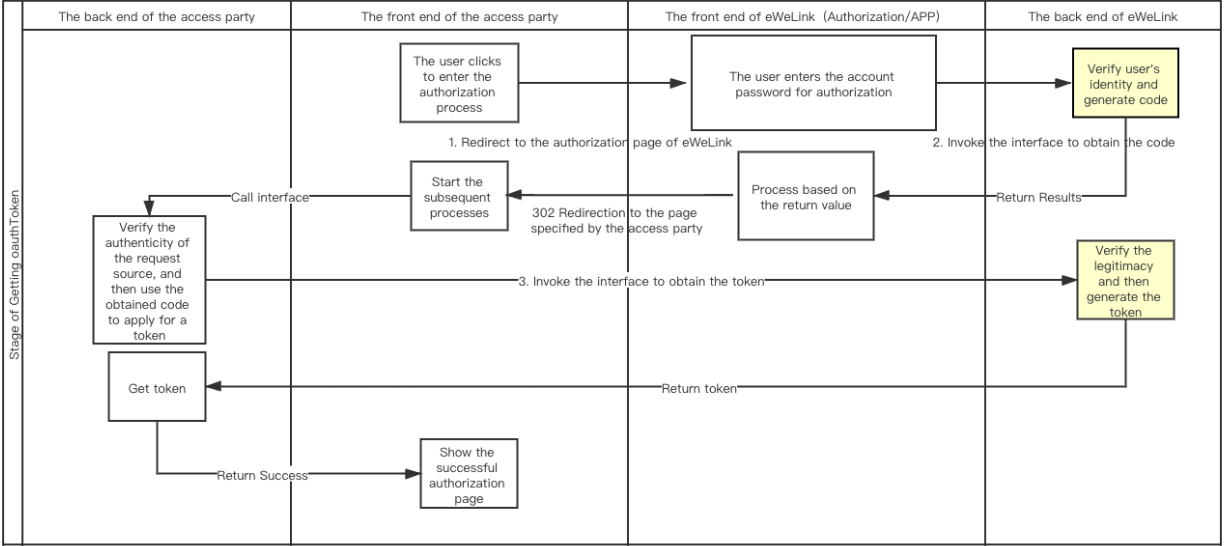
\includegraphics[scale=0.45]{images/cap5/oauth_1.png}
	\end{center}
	\fonte{\cite{COOLKITOAUTH}}
\end{figure}

No contexto da aplicação desenvolvida neste PFC, o usuário é redirecionado para a página de autenticação da eWeLink, onde ele pode inserir suas credenciais. Após o login bem-sucedido, a eWeLink redireciona o usuário de volta ao sistema com um código de autorização (\textit{access token}) conforme demonstrado na \autoref{fig:oauth1}, que é armazenado no banco de dados para permitir interações futuras com a API.

\subsubsubsection{Obtenção do Token de Acesso eWeLink}
\begin{itemize}
    \item \textbf{Rota:} \texttt{GET /ewelink/redirectUrl}
    \item \textbf{Descrição:} Recebe o código de autorização da eWeLink e gera um token de acesso.
    \item \textbf{Fluxo:}
    \begin{enumerate}
        \item O usuário é redirecionado da eWeLink para o sistema com um código de autorização e o id do \textit{tenant}.
        \item O sistema utiliza esse código para obter um token de acesso e um token de atualização.
        \item As credenciais são armazenadas no banco de dados usando o id do \textit{tenant} para permitir interações futuras com a API.
    \end{enumerate}
\end{itemize}

\subsubsubsection{Listagem de Dispositivos eWeLink}
\begin{itemize}
    \item \textbf{Rota:} \texttt{POST /tenants/:tenantId/ewelink/listAllThings}
    \item \textbf{Descrição:} Lista todos os dispositivos associados a um determinado \textit{tenant}.
    \item \textbf{Fluxo:}
    \begin{enumerate}
        \item O usuário autenticado com permissão faz uma requisição para listar os dispositivos.
        \item O serviço verifica as credenciais e atualiza os tokens se necessário.
        \item O serviço consulta a API eWeLink e retorna a lista de dispositivos cadastrados.
    \end{enumerate}
\end{itemize}

\begin{figure}[htp]
	\caption{\label{fig:oauth2}OAuth2.0 EWeLink: Usando um \textit{access token}}
	\begin{center}
	  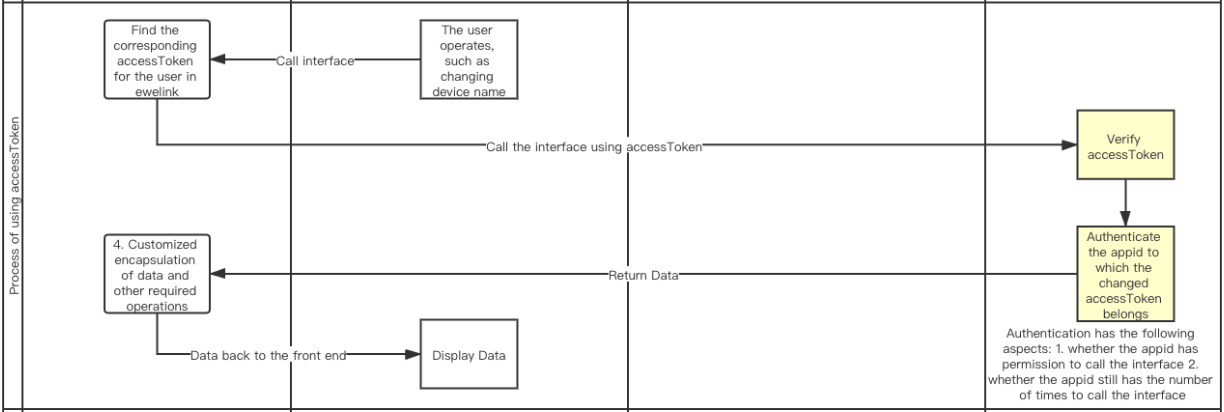
\includegraphics[scale=0.45]{images/cap5/oauth_2.png}
	\end{center}
	\fonte{\cite{COOLKITOAUTH}}
\end{figure}

A \autoref{fig:oauth2} mostra o processo de uso do \textit{access token} na interação com a plataforma \textit{Coolkit Open Platform 4.3 EWeLink}. Neste exemplo, o usuário autenticado com permissão realiza uma requisição para listar os dispositivos, que são consultados na API eWeLink e retornados ao usuário.

\begin{figure}[htp]
	\caption{\label{fig:oauth3}OAuth2.0 EWeLink: Atualizando um \textit{access token}}
	\begin{center}
	  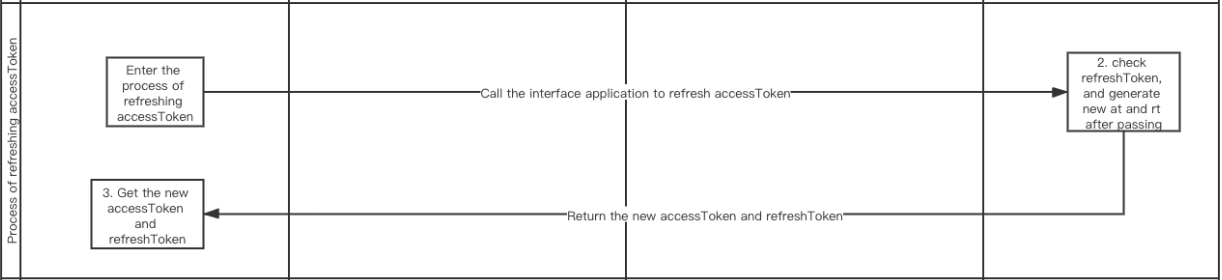
\includegraphics[scale=0.45]{images/cap5/oauth_3.png}
	\end{center}
	\fonte{\cite{COOLKITOAUTH}}
\end{figure}

Caso o \textit{access token} esteja expirado ou inválido, a aplicação solicita um novo token utilizando o \textit{refresh token}. O servidor de autorização gera um novo \textit{access token} e um novo \textit{refresh token}, que podem ser usados para futuras requisições. Caso o \textit{refresh token} esteja expirado ou inválido, a plataforma acusará erro e indicará ao usuário para efetuar login novamente para obter um novo \textit{access token} e \textit{refresh token}.
 
\noindent\textbf{Outras Operações}\\
Além das rotas descritas acima, o módulo também inclui funcionalidades para atualização de tokens de acesso, e controle dos dispositivos IoT para fins de testes (os controles da plataforma serão enviados pelo módulo \textit{schedule} demonstrado na \autoref{subsubsec:envio_comandos_iot}).

\subsubsection{Módulo de Quadras-Dispositivos}\label{subsubsec:modulo_quadras_dispositivos}

\noindent\textbf{Visão Geral}\\
O módulo de \textit{field-devices} é responsável pela integração entre as quadras esportivas e os dispositivos IoT, permitindo o gerenciamento dos equipamentos eletrônicos associados a cada quadra. Essa funcionalidade possibilita o controle automatizado de iluminação, climatização e outros dispositivos conectados, otimizando a experiência do usuário e a gestão operacional do sistema.

As principais funcionalidades deste módulo incluem:

\begin{itemize}
\item Associação de comandos de dispositivos a quadras esportivas específicas.
\item Consulta e listagem dos comandos de dispositivos cadastrados para uma quadra.
\item Atualização e remoção de dispositivos vinculados às quadras.
\item Controle seguro de permissões, garantindo que apenas administradores e gerentes possam gerenciar os dispositivos.
\end{itemize}

\noindent\textbf{Fluxo das Rotas}\\
As rotas deste módulo são definidas no \texttt{FieldDevicesController} e interagem com o serviço de gerenciamento de dispositivos \texttt{FieldDevicesService}. A seguir, são apresentados os fluxos de todas as operações disponíveis.

\subsubsubsection{Criação de um Dispositivo de Quadra}
\begin{itemize}
\item \textbf{Rota:} \texttt{POST /tenants/:tenantId/fields/:fieldId/field-devices}
\item \textbf{Descrição:} Criar um novo comando de dispositivo vinculado a uma quadra esportiva.
\item \textbf{Fluxo:}
\begin{enumerate}
\item O usuário autenticado com permissão faz uma requisição contendo os dados do dispositivo obtidos através da API eWeLink juntamente com o comando desejado.
\item O serviço verifica se a quadra informada existe.
\item Se validado, os dados do dispositivo e o comando desejado são armazenados no banco de dados e associados à quadra.
\item A resposta retorna uma mensagem de sucesso e os detalhes do dispositivo cadastrado.
\end{enumerate}
\end{itemize}

\subsubsubsection{Consulta de Todos os Dispositivos de uma Quadra}
\begin{itemize}
\item \textbf{Rota:} \texttt{GET /tenants/:tenantId/fields/:fieldId/field-devices}
\item \textbf{Descrição:} Retorna uma lista com todos os dispositivos vinculados a uma quadra específica.
\item \textbf{Fluxo:}
\begin{enumerate}
\item O usuário faz uma requisição para listar os dispositivos de uma quadra específica.
\item O serviço busca todos os dispositivos associados à quadra no banco de dados.
\item A lista dos dispositivos cadastrados é retornada na resposta.
\end{enumerate}
\end{itemize}

\subsubsubsection{Consulta de um Dispositivo de Quadra Específico}
\begin{itemize}
\item \textbf{Rota:} \texttt{GET /tenants/:tenantId/fields/:fieldId/field-devices/:id}
\item \textbf{Descrição:} Buscar um dispositivo específico vinculado a uma quadra esportiva.
\item \textbf{Fluxo:}
\begin{enumerate}
\item O usuário faz uma requisição com o identificador do dispositivo e da quadra correspondente.
\item O serviço consulta o banco de dados para localizar o dispositivo correspondente.
\item Se encontrado, os detalhes do dispositivo são retornados na resposta.
\item Se o dispositivo não for encontrado, uma exceção é lançada informando o erro.
\end{enumerate}
\end{itemize}

\subsubsubsection{Atualização de um Dispositivo de Quadra}
\begin{itemize}
\item \textbf{Rota:} \texttt{PATCH /tenants/:tenantId/fields/:fieldId/field-devices/:id}
\item \textbf{Descrição:} Atualiza as informações de um comando de dispositivo vinculado a uma quadra esportiva.
\item \textbf{Fluxo:}
\begin{enumerate}
\item O usuário autenticado com permissão faz uma requisição contendo os dados atualizados do dispositivo.
\item O serviço verifica se o dispositivo informado existe.
\item Se validado, os dados do dispositivo são atualizados no banco de dados.
\item A resposta retorna uma mensagem de sucesso e os detalhes do dispositivo atualizado.
\end{enumerate}
\end{itemize}

\subsubsubsection{Remoção de um Dispositivo de Quadra}
\begin{itemize}
\item \textbf{Rota:} \texttt{DELETE /tenants/:tenantId/fields/:fieldId/field-devices/:id}
\item \textbf{Descrição:} Remove um comando de dispositivo vinculado a uma quadra esportiva.
\item \textbf{Fluxo:}
\begin{enumerate}
\item O usuário autenticado com permissão faz uma requisição para remover o dispositivo.
\item O serviço verifica se o dispositivo informado existe.
\item Se encontrado, o dispositivo é removido logicamente do banco de dados.
\item A resposta confirma a remoção do dispositivo.
\end{enumerate}
\end{itemize}

\subsubsection{Módulo de Reservas e Comandos IoT}\label{subsubsec:modulo_reservas}

\noindent\textbf{Visão Geral}\\
O módulo de \textit{reservas e comandos IoT} é responsável pelo gerenciamento das reservas de quadras esportivas e pela automação dos dispositivos IoT associados. Ele garante que os usuários possam realizar reservas de maneira eficiente, ao mesmo tempo que controla dispositivos como iluminação e climatização, otimizando os recursos disponíveis.

As principais funcionalidades deste módulo incluem:

\begin{itemize}
    \item Criação e gerenciamento de reservas de quadras esportivas.
    \item Listagem de reservas existentes, incluindo filtros por período e usuário.
    \item Controle automatizado de dispositivos IoT com base nos horários das reservas.
    \item Prevenção de conflitos de horários e gerenciamento de comandos consecutivos para dispositivos.
\end{itemize}

\noindent\textbf{Fluxo das Rotas}\\
As rotas deste módulo são definidas no \texttt{BookingsController} e interagem com o serviço de gerenciamento de reservas e automação de dispositivos IoT, fornecido pelo \texttt{BookingsService}. A seguir, são apresentados os fluxos das principais operações disponíveis.

\subsubsubsection{Criação de uma Reserva}
\begin{itemize}
    \item \textbf{Rota:} \texttt{POST /tenants/:tenantId/fields/:fieldId/bookings}
    \item \textbf{Descrição:} Criar uma nova reserva para uma quadra esportiva.
    \item \textbf{Fluxo:}
    \begin{enumerate}
        \item O usuário autenticado com permissão faz uma requisição contendo os detalhes da reserva.
        \item O serviço verifica se a quadra informada existe e se a disponibilidade está correta.
        \item Caso não haja conflitos de horário, a reserva é criada e armazenada no banco de dados.
        \item Se houver dispositivos IoT associados à quadra, são criados comandos automáticos para acioná-los no início e no final da reserva.
        \item A resposta retorna uma mensagem de sucesso com os detalhes da reserva e dos comandos IoT gerados.
    \end{enumerate}
\end{itemize}

O código construído para o o \textit{service} está disponível no \autoref{cod:create-booking-service}.

\subsubsubsection{Listagem de Reservas de uma Quadra}
\begin{itemize}
    \item \textbf{Rota:} \texttt{GET /tenants/:tenantId/fields/:fieldId/bookings}
    \item \textbf{Descrição:} Retorna todas as reservas vinculadas a uma quadra específica.
    \item \textbf{Fluxo:}
    \begin{enumerate}
        \item O usuário faz uma requisição para listar as reservas de uma quadra específica.
        \item O serviço busca todas as reservas associadas à quadra no banco de dados.
        \item A lista das reservas cadastradas é retornada na resposta.
    \end{enumerate}
\end{itemize}

\subsubsubsection{Listagem de Reservas Futuras por Período}
\begin{itemize}
    \item \textbf{Rota:} \texttt{POST /tenants/:tenantId/fields/:fieldId/bookings/future}
    \item \textbf{Descrição:} Retorna todas as reservas futuras dentro de um determinado período.
    \item \textbf{Fluxo:}
    \begin{enumerate}
        \item O usuário faz uma requisição informando um intervalo de tempo desejado.
        \item O serviço busca todas as reservas futuras que se enquadram no período informado.
        \item A resposta retorna uma lista de reservas futuras.
    \end{enumerate}
\end{itemize}

\subsubsubsection{Consulta de uma Reserva Específica}
\begin{itemize}
    \item \textbf{Rota:} \texttt{GET /tenants/:tenantId/fields/:fieldId/bookings/:id}
    \item \textbf{Descrição:} Buscar uma reserva específica dentro de uma quadra esportiva.
    \item \textbf{Fluxo:}
    \begin{enumerate}
        \item O usuário faz uma requisição com o identificador da reserva e da quadra correspondente.
        \item O serviço consulta o banco de dados para localizar a reserva correspondente.
        \item Se encontrada, os detalhes da reserva são retornados na resposta.
        \item Se a reserva não for encontrada, uma exceção é lançada informando o erro.
    \end{enumerate}
\end{itemize}

\subsubsubsection{Cancelamento de uma Reserva}
\begin{itemize}
    \item \textbf{Rota:} \texttt{DELETE /tenants/:tenantId/fields/:fieldId/bookings/:id}
    \item \textbf{Descrição:} Cancela uma reserva existente e remove os comandos IoT associados.
    \item \textbf{Fluxo:}
    \begin{enumerate}
        \item O usuário autenticado faz uma requisição para cancelar uma reserva existente.
        \item O serviço verifica se a reserva existe.
        \item Caso existam comandos IoT pendentes para a reserva, estes são removidos do banco de dados.
        \item A reserva é marcada como cancelada e excluída do banco de dados.
        \item A resposta confirma o cancelamento da reserva e a remoção dos comandos IoT.
    \end{enumerate}
\end{itemize}

\subsubsection{Envio de Comandos IoT}\label{subsubsec:envio_comandos_iot}

\noindent\textbf{Visão Geral}\\
O módulo \textit{schedule} é responsável por garantir o envio dos comandos IoT para a API eWeLink no momento adequado. Para isso, ele utiliza a biblioteca \texttt{@nestjs/schedule}, que permite a execução de tarefas periódicas dentro do sistema. O agendamento periódico verifica comandos pendentes e os envia à API eWeLink, garantindo que os dispositivos IoT sejam acionados conforme as reservas criadas no sistema.

O processo de agendamento é realizado com a anotação \texttt{@Cron('* * * * *')}, que configura a execução da tarefa a cada minuto. Durante essa execução, o sistema:

\begin{itemize}
    \item Consulta os comandos pendentes no banco de dados.
    \item Agrupa os comandos por \textit{tenant}.
    \item Filtra e prioriza os comandos mais recentes para cada dispositivo.
    \item Envia os comandos selecionados à API eWeLink.
    \item Atualiza o status dos comandos no banco de dados.
\end{itemize}

\noindent\textbf{Fluxo de Execução}\\
O módulo segue um fluxo detalhado para processar os comandos de dispositivos IoT de maneira eficiente e segura:

\begin{enumerate}
  \item Consulta de Comandos Pendentes
  \begin{itemize}
      \item O sistema busca no banco de dados os comandos cujo horário de execução já tenha sido alcançado e que ainda estejam no estado \texttt{PENDING}.
      \item Os comandos são agrupados por \textit{tenant} para garantir que cada empresa tenha seus dispositivos controlados separadamente e com uma única chamada à API EWeLink.
  \end{itemize}
  
  \item Filtragem de Comandos Duplicados
  \begin{itemize}
      \item Para cada dispositivo IoT, apenas o comando mais recente é mantido para execução, evitando envio de comandos desnecessários.
      \item Comandos mais antigos para o mesmo dispositivo são marcados como \texttt{SKIPPED} para evitar acionamentos desnecessários.
  \end{itemize}
  
  \item Envio dos Comandos à API eWeLink
  \begin{itemize}
      \item Os comandos selecionados são formatados no padrão aceito pela API eWeLink demonstrado no \autoref{cod:formato_controle_iot}.
      \item O sistema busca e verifica se os \textit{access tokens} de cada empresa estão válidos, caso contrário utiliza os \textit{refresh tokens} para obter um novo \textit{access token} ou emite um erro caso o \textit{refresh token} esteja expirado e continua para os próximos \textit{tenants}.
      \item O sistema envia os comandos em lote para otimizar a comunicação.
      \item A resposta da API é analisada para verificar quais comandos foram executados com sucesso e quais falharam.
  \end{itemize}

  \begin{lstlisting}[caption={Formato de envio de comando para \acrshort{API}.},label={cod:formato_controle_iot}]
    [
      {
        type: 0 | 1,
        id: "<id do dispositivo na plataforma ewelink>",
        params: {
          switch: "on" | "off"
        }
      }
    ]
  \end{lstlisting}

  O serviço desenvolvido para envio dos comandos à \acrshort{API} eWeLink com auxílio da biblioteca \textit{ewelink-api-next} desenvolvida pela \textit{Coolkit} na linguagem javascript está disponível no \autoref{cod:envio_comandos_iot}.

  \begin{lstlisting}[caption={Serviço para envio de comandos IoT à \acrshort{API} eWeLink.},label={cod:envio_comandos_iot}]
    async controlBatchThing(tenantId: string, thingList: SetThingDto[]) {
    const { accessToken, region } =
      await this.checkAccessAndRefreshToken(tenantId)

    this.client.at = accessToken
    this.client.region = region
    this.client.setUrl(region)

    const response = await this.client.device.setAllThingStatus({ thingList })

    return response
  }
  \end{lstlisting}
  
  \item Atualização do Status dos Comandos
  \begin{itemize}
      \item Os comandos que foram executados com sucesso são marcados como \texttt{EXECUTED}.
      \item Os comandos que falharam na execução são marcados como \texttt{FAILED}.
      \item Em caso de erro geral na execução, todos os comandos do \textit{tenant} são atualizados para \texttt{FAILED}.
  \end{itemize}
\end{enumerate}

\noindent\textbf{Conclusão}\\
O módulo \textit{schedule} desempenha um papel fundamental na automação dos dispositivos IoT integrados ao sistema. Ao utilizar a biblioteca \texttt{@nestjs/schedule}, garante-se que os comandos sejam processados no momento correto, evitando acionamentos incorretos e otimizando a interação com a API eWeLink. Essa abordagem melhora a eficiência operacional do sistema e proporciona uma experiência mais confiável para o envio de comandos ao dispositivos IoT.

\section{Análise de Resultados}\label{sec:analise_resultados}

Esta seção apresenta uma análise detalhada dos resultados obtidos com a implementação do sistema de gerenciamento de reservas de quadras esportivas e automação de dispositivos IoT. A avaliação se baseia em indicadores de desempenho, gráficos e estatísticas para determinar a eficácia da solução desenvolvida em comparação com métodos anteriores.

\subsection{Avaliação dos Resultados}

A implementação realizada solucionou o problema tratado ao fornecer uma aplicação de servidor eficiente para o agendamento de quadras esportivas e o controle automatizado de dispositivos IoT com fácil configuração através da integração com a plataforma EWeLink. Os resultados obtidos foram analisados a partir dos seguintes aspectos:

\subsubsection{Eficiência e Desempenho}

O novo sistema demonstrou desempenho significativo no processo de reservas e na automação de dispositivos. Através de uma bateria de testes realizados através de um script automatizado para envio de diversas requisições, foi observado que o sistema foi capaz de manter velocidade média de resposta das requisições inferior à 2 segundos para as principais funcionalidades analisadas em um ambiente de testes local com hardware de nível intermediário presente na \autoref{tab:hardware_teste_local}. As chamadas foram realizadas de um outro computador através da rede local, a fim de simular um ambiente real.

\begin{table}[htb]
	\centering
	\caption{\label{tab:hardware_teste_local}Hardware de testes utilizado na análise de desempenho do sitema.}	
	\begin{tabular}{|l|c|p{6cm}|}
		\hline
		\textbf{Dispositivo} & \textbf{marca} & \textbf{modelo} \\ \hline
    Processador & AMD & Ryzen 5 3600 \\ \hline
    Placa-mãe & Gigabyte & B450M DS3H V2 \\ \hline
    Placa de vídeo & Gigabyte & RTX3070 Aorus Master \\ \hline
    Memória RAM & XPG & 4x8GB DDR4 3000MHz \\ \hline
    SSD & KingDian & 512GB NVME read/write speed 2500MB/s | 1500MB/s\\ \hline
	\end{tabular}
	\fonte{Autor.}
\end{table}

O código base desenvolvido para realiza n chamadas ao \textit{endpoit} e calcular o tempo médio de resposta está apresentado no \autoref{cod:script_tempo_medio_resposta}.

\begin{lstlisting}[caption={\textit{script} para cálculo do tempo médio de resposta.},label={cod:script_tempo_medio_resposta}]
  const axios = require('axios');

  const sendRequest = (startTime, i) => {
    const timePromise = new Promise(resolve => {
        axios.get(url, {headers: headerWithAccessToken});
        const responseTime = Date.now() - startTime;
        console.log(`Request ${i + 1} took ${responseTime} ms`)
        resolve(responseTime)
    })
    return timePromise
  }

  const headerWithAccessToken = {
    headers: {
      'Authorization': `Bearer ACCESS_TOKEN`
    }
  }
  
  async function measureAverageResponseTime(url, n) {
    let promises = []
  
    for (let i = 0; i < n; i++) {
      const start = Date.now();
      try {
        const timePromise = sendRequest(start, i)
        promises.push(timePromise)
      } catch (error) {
        console.error(`Request ${i + 1} failed:`, error.message);
      }
    }
    const resolvedTimes = await Promise.all(promises)
    const totalTime = resolvedTimes.reduce((acc, curr) => acc + curr, 0)

    const averageResponseTime = totalTime / n;
    console.log(`Average response time over ${n} requests: ${averageResponseTime.toFixed(0)} ms`);
  }
  
  // Example usage:
  const apiUrl = 'http://localhost:3000/tenants/451e6db3-1a94-4918-9ec1-b8aa793f0269/fields/5b7a652f-0ddb-4a52-b552-4f92a02026d2/bookings'; // To get all bookings from a field
  const numberOfCalls = 1000;
  
  measureAverageResponseTime(apiUrl, numberOfCalls);
\end{lstlisting}

Para alguns \textit{endpoints} foi necessário realizas algumas modificações no código para garantir que ele funcionasse corretamente. Por exemplo, alguns endpoints exigiam autenticação e outros não. Além disso, alguns endpoints exigiam parâmetros específicos na requisição, como e-mails, senhas e outros dados, sendo necessário criar listas com parâmetros \textit{mockados}. Com os \textit{scripts} de teste prontos, foi possível realizar a análise dos principais endpoints do sistema realizando 1000 chamadas para cada e calcular o tempo médio de resposta.

\begin{table}[htb]
  \centering
  \caption{\label{tab:tempo_medio_resposta}Tempo médio de resposta para os principais \textit{endpoints} analisados.}
  \begin{tabular}{|m{6cm}|c|p{4cm}|c|}
  \hline
  \textbf{Enpoint} & \textbf{método} & \textbf{descrição} & \textbf{tempo (ms)} \\ \hline
  /auth/login & POST & login de usuário & 12 \\ \hline
  /auth/register & POST & Registra um novo usuario & 174 \\ \hline
  /auth/refresh & GET & Renova o token de acesso & 52 \\ \hline
  /users & GET & Lista todos os usuarios & 204 \\ \hline
  /tenants & GET & Lista todos os tenants & 124 \\ \hline
  % \multicolumn{4}{|c|}{\textbf{/tenants/:tenantId/fields}} \\ \hline
  \textbf{/tenants/:tenantId/fields} & & & \\ \hline
  / & GET & Lista todas as quadras de um\textit{tenant}& 155 \\ \hline
  /:id & GET & Retorna os detalhes de uma quadra especifica & 73 \\ \hline
  /:fieldId/field-availabilities & GET & Lista as disponibilidades de uma quadra & 212 \\ \hline
  /:fieldId/bookings & POST & Cria uma nova reserva & 230 \\ \hline
  /:fieldId/bookings & GET & Lista todas as reservas de uma quadra & 344 \\ \hline
  /:fieldId/bookings/future & POST & Lista reservas futuras & 281 \\ \hline
  /:fieldId/bookings/future-by-user & POST & Lista reservas futuras por usuario & 292 \\ \hline
  /:fieldId/bookings/:id & GET & Retorna os detalhes de uma reserva especifica & 125 \\ \hline
  /:fieldId/field-devices & GET & Lista todos os dispositivos de uma quadra & 123 \\ \hline
  /:fieldId/field-devices/:id & GET & Retorna os detalhes de um dispositivo & 89 \\ \hline
  \end{tabular}
  \fonte{Autor.}
\end{table}

A \autoref{tab:tempo_medio_resposta} apresenta o tempo médio de resposta para cada um dos principais e mais críticos endpoints da \acrshort{API}. Esses resultados comprovam a eficiência e desempenho do novo sistema em gerenciar reservas de quadras e controlar dispositivos IoT, demonstrando sua capacidade de atender às necessidades dos usuários e melhorar a experiência de locação, além de atender os requisitos técnicos desejados e definidos no início do projeto. Apesar do ambiente testado ter sido local, acredita-se que o sistema será capaz de seguir os requisitos mesmo quando estiver executando em um servidor remoto, pois houve uma boa margem de segurança do resquisito técnico desejado em relação ao tempo médio das chamadas obtido.

\subsection{Vantagens e Desvantagens da Solução Desenvolvida}

\noindent\textbf{Vantagens}\\
\begin{itemize}
    \item Integração direta com a API eWeLink para controle de dispositivos IoT.
    \item Simplicidade na aquisição, instalação, configuração e controle dos dispositivos IoT. 
    \item Gestão eficiente de múltiplos \textit{tenants} em um ambiente unificado.
    \item Redução do consumo de energia elétrica com acionamento automatizado dos dispositivos apenas nos horários de uso.
    \item Segurança aprimorada por meio de autenticação baseada em tokens e controle de permissões de acesso baseado em papéis.
\end{itemize}

\noindent\textbf{Desvantagens}\\
\begin{itemize}
    \item Dependência da conectividade com a API eWeLink para a operação dos dispositivos IoT.
    \item Possível curva de aprendizado para novos usuários e administradores do sistema.
    \item Necessidade de manutenção e melhorias contínuas para atualização necessidades das empresas.
\end{itemize}

\subsection{Problemas Encontrados}

Durante a implementação, alguns desafios técnicos foram identificados, como a necessidade de lidar com comandos IoT duplicados ou atrasados e a otimização do processamento de comandos para evitar sobrecarga no sistema. Além disso, questões relacionadas à conectividade da API eWeLink impactaram levemente na confiabilidade da automação dos dispositivos pois, em alguns momentos, a API pode ficar indisponível ou apresentar lentidão no envio dos comandos aos dispositivos. Embora essa lentidão ocorra, o impacto não deve ser significativo, pois em nenhum caso o envio de comandos demorou mais de 20 segundos para ser efetivado.

\subsection{Impacto dos Resultados Obtidos}

Através de testes simulados, notou-se que a futura implementação do sistema completo trará impactos significativos nos processos e serviços das empresas clientes, com destaque para os seguintes aspectos:

\textbf{Impactos Organizacionais}\\
\begin{itemize}
    \item Maior controle sobre a gestão de reservas e utilização dos espaços esportivos.
    \item Melhoria na comunicação com clientes devido à transparência na disponibilidade de horários.
\end{itemize}

\textbf{Impactos Tecnológicos}\\
\begin{itemize}
    \item Utilização de tecnologias modernas como \textit{NestJS}, \textit{PostgreSQL} e \textit{TypeORM}.
    \item Integração bem-sucedida com dispositivos IoT para automação.
\end{itemize}

\textbf{Impactos Financeiros}\\
\begin{itemize}
    \item Redução de custos operacionais com a automação do acionamento de dispositivos elétricos.
    \item Potencial aumento da receita devido à otimização do uso das quadras.
\end{itemize}

\textbf{Impactos Ecológicos}\\
\begin{itemize}
    \item Redução do consumo de energia elétrica por meio da automação dos dispositivos IoT.
    \item Contribuição para práticas mais sustentáveis no gerenciamento dos espaços esportivos.
\end{itemize}

\noindent\textbf{Conclusão}\\
A análise dos resultados demonstra que o sistema \textit{backend} desenvolvido atendeu aos objetivos propostos e trouxe melhorias significativas para a gestão de reservas e automação de dispositivos IoT em ambiente simulado. Apesar dos desafios encontrados, a implementação se mostrou eficaz e com grande potencial de expansão e aprimoramento futuro.

% ---

% ---
% 6 - Conclusão
% ---
%\phantompart
% ----------------------------------------------------------
\chapter{Conclusão}\label{cap:conclusao}
% ----------------------------------------------------------

% \textbf{Instruções da Coordenação do PFC:}

% A Conclusão deve apresentar:
% \begin{itemize}
% 	\item Uma \textbf{síntese} do problema tratado, da solução proposta e dos principais resultados obtidos;
% 	\item Uma discussão sobre o que foi atingido no PFC em relação aos objetivos inicialmente traçados e sobre as limitações encontradas;
% 	\item Uma discussão sobre possíveis aprimoramentos;
% 	\item Destacar os impactos do PFC para a empresa/clientes da empresa/instituto de pesquisa, além de possíveis impactos organizacionais, tecnológicos, financeiros, éticos, ecológicos, etc. 
% 	\item Sugestão de trabalhos futuros (como se poderia dar continuidade ao PFC; aplicar o desenvolvimento realizado no PFC a outros problemas/processos; etc)
% \end{itemize}

\section{Síntese do Problema e Solução Proposta}


Com a crescente demanda por alugueis de quadras esportivas e a difusão do uso de dispositivos \acrshort{IoT} para controle de equipamentos elétricos e eletrônicos, surge a necessidade de uma solução robusta que permitisse a simplificação do processo de reserva de quadras e o controle dos equipamentos associados de maneira automatizada.
A Fischertec Tecnologia, buscando reduzir sua dependência de projetos de terceiros e analisando os desafios enfrentados pelas empresas na gestão de reservas de quadras esportivas e no controle automatizado de dispositivos \acrshort{IoT}, decidiu investir em uma solução própria para atender a essas necessidades do setor esportivo.

Este \acrshort{PFC} teve como objetivo solucionar os desafios enfrentados na gestão de reservas de quadras esportivas e no controle automatizado de dispositivos \acrshort{IoT}. Para isso, foi proposto o desenvolvimento de um sistema web multi-tenant que permitisse o gerenciamento eficiente de reservas e a automação de dispositivos inteligêntes conectados via API eWeLink. A solução proposta incluiu um backend robusto desenvolvido com tecnologias modernas como Nest.js, um frontend intuitivo (que será desenvolvido em um futuro próximo) e uma integração eficiente e de fácil configuração com dispositivos \acrshort{IoT}, garantindo maior controle e otimização dos recursos.

\section{Avaliação dos Objetivos e Limitações Encontradas}

Os objetivos inicialmente traçados foram amplamente alcançados, com a criação de um sistema backend funcional e eficiente para gestão de quadras e automação \acrshort{IoT}. A aplicação atendeu a todos os requisitos funcionais e não funcionais definidos nas Seções \ref{subsec:requisitos_funcionais} e \ref{subsec:requisitos_nao_funcionais}, respectivamente, proporcionando um ambiente seguro, escalável e acessível para os usuários.

Entretanto, algumas limitações foram identificadas ao longo do desenvolvimento. A dependência da API eWeLink para o controle dos dispositivos \acrshort{IoT} trouxe preocupações quanto à estabilidade da comunicação, custos de use e manutenção e o tempo de resposta das operações.

\section{Possíveis Aprimoramentos}

Para tornar a solução ainda mais eficiente, algumas melhorias podem ser exploradas no futuro:

\begin{itemize}
  \item Implementação de suporte a múltiplas APIs de dispositivos \acrshort{IoT}, reduzindo a dependência da eWeLink. Uma opção seria a integração com outras plataformas como Tuya, SmartLife, SmartThings e HomeAssistant.
  \item Otimização das consultas ao banco de dados para melhorar o desempenho do sistema, utilizando paginação para rotas com muitos registros.
  \item Uso de \acrfull{LLMs} para criação de relatórios detalhados sobre o uso das quadras e o consumo de energia.
  \item Desenvolvimento de um painel administrativo para monitoramento e controle em tempo real dos dispositivos.
\end{itemize}

\section{Sugestão de Trabalhos Futuros}

Para dar continuidade ao trabalho desenvolvido nesta \acrshort{PFC}, algumas direções podem ser exploradas:

\begin{itemize}
  \item Desenvolvimento da aplicação web frontend para interação com o sistema já desenvolvido. Essa etapa acontecerá em uma etapa subsequente da \acrshort{PFC}.
  \item Desenvolvimento de um aplicativo móvel para facilitar o acesso ao sistema pelos clientes e administradores.
  \item Implementação de um módulo de notificações push para alertar os usuários sobre eventos importantes, como agendamentos próximos ou alterações no status dos dispositivos.
  \item Customização do sistema para atender aulas em grupo, com quantidade de vagas e associação de vários usuários ao agendamento.
  \item Desenvolvimento de um módulo de análise de dados para fornecer relatórios detalhados sobre a utilização das quadras.
  \item Integração com sistemas de pagamento online para facilitar a gestão financeira das reservas.
\end{itemize}

O desenvolvimento deste PFC demonstrou a viabilidade e os benefícios de uma solução integrada para a gestão de reservas de quadras esportivas e automação \acrshort{IoT}. Apesar dos desafios encontrados, os resultados obtidos comprovam a eficiência da abordagem adotada e abrem espaço para futuras melhorias e expansões. A criação de um sistema próprio representa um avanço para a Fischertec, permitindo maior autonomia através de faturamento recorrente além de levar ao mercado uma solução robusta que atenda às necessidades das empresas do setor esportivo.

% ----------------------------------------------------------
% ELEMENTOS PÓS-TEXTUAIS
% ----------------------------------------------------------
\postextual{}
% ----------------------------------------------------------

% ----------------------------------------------------------
% Referências bibliográficas
% ----------------------------------------------------------
\begingroup
	\printbibliography[title=REFERÊNCIAS]
\endgroup

% ----------------------------------------------------------
% Glossário
% ----------------------------------------------------------
%
% Consulte o manual da classe abntex2 para orientações sobre o glossário.
%
%\glossary

% ----------------------------------------------------------
% Apêndices
% ----------------------------------------------------------

% ---
% Inicia os apêndices
% ---
\begin{apendicesenv}
%	\partapendices* 
	% ----------------------------------------------------------
% \chapter{Descrição 1}
% % ----------------------------------------------------------

% Textos elaborados pelo autor, a fim de completar a sua argumentação. Deve ser precedido da palavra APÊNDICE, identificada por letras maiúsculas consecutivas, travessão e pelo respectivo título. Utilizam-se letras maiúsculas dobradas quando esgotadas as letras do alfabeto. 

\chapter{APÊNDICE A - Código do Controlador}

\begin{lstlisting}[caption={\textit{Service} para a rota de criação de \textit{booking} (agendamento).},label={cod:create-booking-service}]
	async create(
    createBookingDto: CreateBookingDto,
    fieldId: string,
    userId: string
  ) {
    const fieldAvailability = await this.fieldAvailabilitiesService.findOne(
      fieldId,
      createBookingDto.fieldAvailabilityId
    )

    const user = await this.usersService.findById(userId)

    const startDateTime = moment(createBookingDto.startTime)
    const endDateTime = moment(createBookingDto.endTime)
    console.log('startDateTime moment', startDateTime)
    console.log('endDateTime moment', endDateTime)

    const hasConflict = await this.hasBookingConflict(
      fieldId,
      createBookingDto.startTime,
      createBookingDto.endTime
    )

    if (hasConflict)
      throw new ConflictException('Ja existe uma reserva neste periodo')

    // check if the week days are the same
    if (
      startDateTime.utc().day() !==
      moment().day(fieldAvailability.dayOfWeek).day()
    )
      throw new BadRequestException(
        'Dia da semana solicitado nao confere com o dia disponivel'
      )

    // check if the start and end times match the availability range
    if (
      startDateTime.utc().format('HH:mm:ss') !== fieldAvailability.startTime ||
      endDateTime.utc().format('HH:mm:ss') !== fieldAvailability.endTime
    ) {
      console.log('hora disponivel inicio:', fieldAvailability.startTime)
      console.log(
        'hora solicitada inicio:',
        startDateTime.utc().format('HH:mm:ss')
      )
      console.log('hora disponivel final:', fieldAvailability.endTime)
      console.log(
        'hora solicitada final:',
        endDateTime.utc().format('HH:mm:ss')
      )

      throw new BadRequestException(
        'Horarios solicitados nao conferem com os horarios disponiveis'
      )
    }

    const booking = new Booking()

    Object.assign(booking, {
      ...createBookingDto,
      field: fieldAvailability.field,
      user
    } as unknown as Booking)
    // Filter data to return without user for the booking
    const createdBooking = await this.bookingsRepository.save(booking)

    const fieldDevicesByField = await this.fieldDevicesService.findAll(fieldId)

    // if there are field devices, create device commands
    const returnObject = { booking: createdBooking }
    if (fieldDevicesByField.length > 0) {
      const bookingDeviceCommands = fieldDevicesByField.map((device) => {
        const deviceCommand = new DeviceCommand()
        Object.assign(deviceCommand, {
          booking: createdBooking,
          fieldDevice: device,
          executionTime:
            device.eventType === EventTypeEnum.START
              ? booking.startTime
              : booking.endTime
        })
        return deviceCommand
      })

      const consecutiveCommands = await Promise.all(
        bookingDeviceCommands.map((command) => {
          // Step 1: Check if there are any consecutive commands for the same device and ignore them
          const query = {
            where: {
              status: CommandStatusEnum.PENDING,
              fieldDevice: {
                deviceId: command.fieldDevice.deviceId,
                skipIfConsecutive: true,
                field: { id: fieldId }
              },
              executionTime: Between(
                moment(command.executionTime).subtract(5, 'minutes').toDate(),
                moment(command.executionTime).add(5, 'minutes').toDate()
              )
            },
            relations: { fieldDevice: { field: true } }
          }
          return this.deviceCommandsRepository.findOne(query)
        })
      )

      // search if the command has any consecutive command so it needs to be ignored
      const deviceCommandsWithoutConsecutiveCommands =
        bookingDeviceCommands.filter(
          (_command, index) => !consecutiveCommands[index]
        )

      // delete the pending commands that are already in the device_command table
      const commandsToDeleteFromDeviceCommandTable = consecutiveCommands.filter(
        (command) => !!command
      )

      // delete the commands from the device_command table
      if (commandsToDeleteFromDeviceCommandTable.length > 0) {
        await this.deviceCommandsRepository.delete(
          commandsToDeleteFromDeviceCommandTable.map((command) => command.id)
        )

        returnObject['deviceCommandsDeleted'] =
          commandsToDeleteFromDeviceCommandTable
      }
      returnObject['deviceCommandsCreated'] =
        await this.deviceCommandsRepository.save(
          deviceCommandsWithoutConsecutiveCommands
        )
    }

    return returnObject
  }

  async hasBookingConflict(
    fieldId: string,
    startTime: string,
    endTime: string
  ): Promise<boolean> {
    const conflict = await this.bookingsRepository.query(
      `SELECT COUNT(*) > 0 AS has_overlap
      FROM booking
      WHERE "fieldId" = $1
        AND "startTime" < $3
        AND "endTime" > $2`,
      [fieldId, startTime, endTime]
    )
    return conflict[0]?.has_overlap
  }
\end{lstlisting}
\end{apendicesenv}
% ---


% ----------------------------------------------------------
% Anexos
% ----------------------------------------------------------

% ---
% Inicia os anexos
% ---
\begin{anexosenv}
%	\partanexos*
	% ----------------------------------------------------------
\chapter{Descrição 2}
% ----------------------------------------------------------

São documentos não elaborados pelo autor que servem como fundamentação (mapas, leis, estatutos). Deve ser precedido da palavra ANEXO, identificada por letras maiúsculas consecutivas, travessão e pelo respectivo título. Utilizam-se letras maiúsculas dobradas quando esgotadas as letras do alfabeto. 

\end{anexosenv}

%---------------------------------------------------------------------
% INDICE REMISSIVO
%---------------------------------------------------------------------
%\phantompart
%\printindex
%---------------------------------------------------------------------

\end{document}
